\documentclass[11pt]{article}
\usepackage[utf8]{inputenc}
\usepackage[T1]{fontenc}
\usepackage{textcomp}
\usepackage[a4paper,margin=2.1cm]{geometry}
\usepackage{amsmath,amssymb}
\usepackage{tikz}
\usepackage{xcolor}
\usepackage{mdframed}
\usepackage{enumitem}
\usepackage[colorlinks=true,linkcolor=blue!60!black]{hyperref}
\setlength{\parindent}{0pt}
\setlength{\parskip}{6pt}

\newcommand{\question}[1]{\par\medskip\noindent\textbf{#1}\par}
\newmdenv[linecolor=green!45!black,linewidth=0.8pt,backgroundcolor=green!4,
  innertopmargin=4pt,innerbottommargin=4pt,skipabove=6pt,skipbelow=6pt]{answerbox}

\title{\textbf{Factorising}\\[0.3em]\large Worked Solutions with Area-Model Diagrams}
\author{Wisest Maths --- Year 1 A-Level, Algebra (ref \texttt{a2})}
\date{}

\begin{document}
\maketitle
\noindent This document contains all 50 \emph{Factorising} questions, each with a fully worked
solution and a TikZ \emph{area-model} (box-method) diagram. Factorising is expanding run \emph{in reverse}:
the terms of the expression are placed \emph{inside} the grid, and the factors are read off the
\emph{edges}. For a common factor the grid is a single row (the factor down the side, the bracket along
the top); for a difference of two squares it is a $2\times2$ grid in which the two off-diagonal terms
cancel; for grouping the four given terms are exactly the four interior cells.
\tableofcontents
\bigskip
\hrule

\section*{Factorising 1\quad\small\texttt{(a2-001)}}
\addcontentsline{toc}{section}{Factorising 1 (a2-001)}
\textit{Difficulty: Foundation \quad\textbar\quad Marks: 2}

\question{Factorise: \( 14m +21n \)}

\textbf{Worked solution.}

\textit{The highest common factor of 14 and 21 is 7.}
\[\begin{gathered}
7(2m+3n)
\end{gathered}\]
Look for highest common factors (HCF).

\begin{answerbox}
\textbf{Final answer:}\quad \(\displaystyle 7(2m+3n)\)
\end{answerbox}
\textbf{Area-model diagram.}

\begin{center}
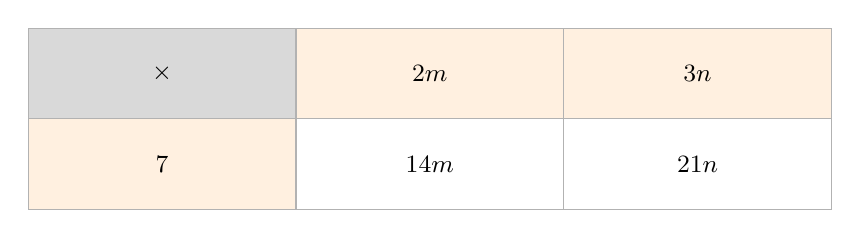
\begin{tikzpicture}[x=1cm,y=1cm,every node/.style={font=\small}]
\fill[gray!30] (0,0) rectangle (3.4,-1.15);
\draw[gray!60] (0,0) rectangle (3.4,-1.15);
\node at (1.7,-0.575) {$\displaystyle \times$};
\fill[orange!12] (3.4,0) rectangle (6.8,-1.15);
\draw[gray!60] (3.4,0) rectangle (6.8,-1.15);
\node at (5.1,-0.575) {$\displaystyle 2m$};
\fill[orange!12] (6.8,0) rectangle (10.2,-1.15);
\draw[gray!60] (6.8,0) rectangle (10.2,-1.15);
\node at (8.5,-0.575) {$\displaystyle 3n$};
\fill[orange!12] (0,-1.15) rectangle (3.4,-2.3);
\draw[gray!60] (0,-1.15) rectangle (3.4,-2.3);
\node at (1.7,-1.725) {$\displaystyle 7$};
\fill[white] (3.4,-1.15) rectangle (6.8,-2.3);
\draw[gray!60] (3.4,-1.15) rectangle (6.8,-2.3);
\node at (5.1,-1.725) {$\displaystyle 14m$};
\fill[white] (6.8,-1.15) rectangle (10.2,-2.3);
\draw[gray!60] (6.8,-1.15) rectangle (10.2,-2.3);
\node at (8.5,-1.725) {$\displaystyle 21n$};
\end{tikzpicture}
\end{center}
\small HCF $7$ down the side; read the other factor $(2m+3n)$ across the top.\normalsize

\medskip\hrule

\section*{Factorising 2\quad\small\texttt{(a2-002)}}
\addcontentsline{toc}{section}{Factorising 2 (a2-002)}
\textit{Difficulty: Foundation \quad\textbar\quad Marks: 2}

\question{Factorise: \( 5x^3y^2 - 15x^2y^3 \)}

\textbf{Worked solution.}

\textit{The highest common factor (HCF) of 5 and 15 is 5. The highest common power of \( x\) is \( x^2 \), and for \( y\) it is \(y^2\).}
\[\begin{gathered}
5x^2y^2(x-3y)
\end{gathered}\]
Identify the highest common factors in the expression.

\begin{answerbox}
\textbf{Final answer:}\quad \(\displaystyle 5x^2y^2(x-3y)\)
\end{answerbox}
\textbf{Area-model diagram.}

\begin{center}
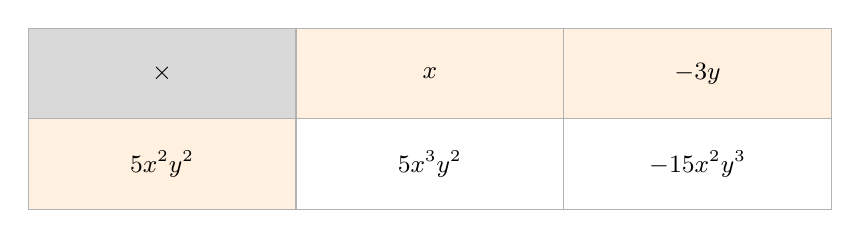
\begin{tikzpicture}[x=1cm,y=1cm,every node/.style={font=\small}]
\fill[gray!30] (0,0) rectangle (3.4,-1.15);
\draw[gray!60] (0,0) rectangle (3.4,-1.15);
\node at (1.7,-0.575) {$\displaystyle \times$};
\fill[orange!12] (3.4,0) rectangle (6.8,-1.15);
\draw[gray!60] (3.4,0) rectangle (6.8,-1.15);
\node at (5.1,-0.575) {$\displaystyle x$};
\fill[orange!12] (6.8,0) rectangle (10.2,-1.15);
\draw[gray!60] (6.8,0) rectangle (10.2,-1.15);
\node at (8.5,-0.575) {$\displaystyle -3y$};
\fill[orange!12] (0,-1.15) rectangle (3.4,-2.3);
\draw[gray!60] (0,-1.15) rectangle (3.4,-2.3);
\node at (1.7,-1.725) {$\displaystyle 5x^2y^2$};
\fill[white] (3.4,-1.15) rectangle (6.8,-2.3);
\draw[gray!60] (3.4,-1.15) rectangle (6.8,-2.3);
\node at (5.1,-1.725) {$\displaystyle 5x^3y^2$};
\fill[white] (6.8,-1.15) rectangle (10.2,-2.3);
\draw[gray!60] (6.8,-1.15) rectangle (10.2,-2.3);
\node at (8.5,-1.725) {$\displaystyle -15x^2y^3$};
\end{tikzpicture}
\end{center}
\small HCF is $5x^2y^2$ (lowest power of each variable).\normalsize

\medskip\hrule

\section*{Factorising 3\quad\small\texttt{(a2-003)}}
\addcontentsline{toc}{section}{Factorising 3 (a2-003)}
\textit{Difficulty: Foundation \quad\textbar\quad Marks: 2}

\question{Factorise completely: \( 4a^2bc + 12ab^2c - 8abc^2 \)}

\textbf{Worked solution.}

\textit{Step 1: The HCF of the numbers (4, 12, 8) is 4. The common variables are \( a \), \( b \), and \( c \).}
\[\begin{gathered}
4abc
\end{gathered}\]
Identify the highest common numerical and algebraic factors in the expression.

\textit{Step 2: Factor out the HCF from each term in the expression.}
\[\begin{gathered}
4abc(a + 3b - 2c)
\end{gathered}\]
Divide each term by the common factor to find the contents of the bracket.

\begin{answerbox}
\textbf{Final answer:}\quad \(\displaystyle 4abc(a + 3b - 2c)\)
\end{answerbox}
\textbf{Area-model diagram.}

\begin{center}
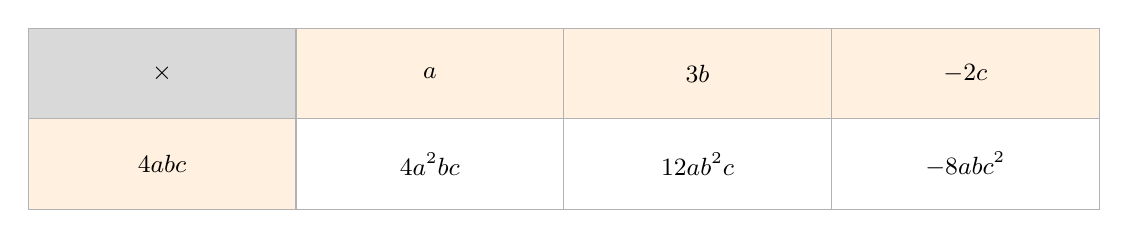
\begin{tikzpicture}[x=1cm,y=1cm,every node/.style={font=\small}]
\fill[gray!30] (0,0) rectangle (3.4,-1.15);
\draw[gray!60] (0,0) rectangle (3.4,-1.15);
\node at (1.7,-0.575) {$\displaystyle \times$};
\fill[orange!12] (3.4,0) rectangle (6.8,-1.15);
\draw[gray!60] (3.4,0) rectangle (6.8,-1.15);
\node at (5.1,-0.575) {$\displaystyle a$};
\fill[orange!12] (6.8,0) rectangle (10.2,-1.15);
\draw[gray!60] (6.8,0) rectangle (10.2,-1.15);
\node at (8.5,-0.575) {$\displaystyle 3b$};
\fill[orange!12] (10.2,0) rectangle (13.6,-1.15);
\draw[gray!60] (10.2,0) rectangle (13.6,-1.15);
\node at (11.9,-0.575) {$\displaystyle -2c$};
\fill[orange!12] (0,-1.15) rectangle (3.4,-2.3);
\draw[gray!60] (0,-1.15) rectangle (3.4,-2.3);
\node at (1.7,-1.725) {$\displaystyle 4abc$};
\fill[white] (3.4,-1.15) rectangle (6.8,-2.3);
\draw[gray!60] (3.4,-1.15) rectangle (6.8,-2.3);
\node at (5.1,-1.725) {$\displaystyle 4a^2bc$};
\fill[white] (6.8,-1.15) rectangle (10.2,-2.3);
\draw[gray!60] (6.8,-1.15) rectangle (10.2,-2.3);
\node at (8.5,-1.725) {$\displaystyle 12ab^2c$};
\fill[white] (10.2,-1.15) rectangle (13.6,-2.3);
\draw[gray!60] (10.2,-1.15) rectangle (13.6,-2.3);
\node at (11.9,-1.725) {$\displaystyle -8abc^2$};
\end{tikzpicture}
\end{center}
\small HCF $4abc$; the bracket has three terms.\normalsize

\medskip\hrule

\section*{Factorising 4\quad\small\texttt{(a2-004)}}
\addcontentsline{toc}{section}{Factorising 4 (a2-004)}
\textit{Difficulty: Foundation \quad\textbar\quad Marks: 2}

\question{Write the expression as a product of factors: \( p^2 - 16q^2 \)}

\textbf{Worked solution.}

\textit{Recognise that the expression is a difference of two squares, where \( 16q^2 \) is \( (4q)^2 \).}
\[\begin{gathered}
p^2 - (4q)^2
\end{gathered}\]
Identify the squared terms.

\begin{answerbox}
\textbf{Final answer:}\quad \(\displaystyle (p - 4q)(p + 4q)\)
\end{answerbox}
\textbf{Area-model diagram.}

\begin{center}
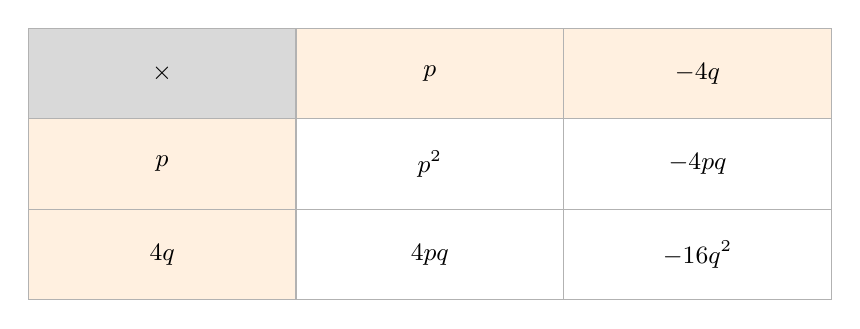
\begin{tikzpicture}[x=1cm,y=1cm,every node/.style={font=\small}]
\fill[gray!30] (0,0) rectangle (3.4,-1.15);
\draw[gray!60] (0,0) rectangle (3.4,-1.15);
\node at (1.7,-0.575) {$\displaystyle \times$};
\fill[orange!12] (3.4,0) rectangle (6.8,-1.15);
\draw[gray!60] (3.4,0) rectangle (6.8,-1.15);
\node at (5.1,-0.575) {$\displaystyle p$};
\fill[orange!12] (6.8,0) rectangle (10.2,-1.15);
\draw[gray!60] (6.8,0) rectangle (10.2,-1.15);
\node at (8.5,-0.575) {$\displaystyle -4q$};
\fill[orange!12] (0,-1.15) rectangle (3.4,-2.3);
\draw[gray!60] (0,-1.15) rectangle (3.4,-2.3);
\node at (1.7,-1.725) {$\displaystyle p$};
\fill[white] (3.4,-1.15) rectangle (6.8,-2.3);
\draw[gray!60] (3.4,-1.15) rectangle (6.8,-2.3);
\node at (5.1,-1.725) {$\displaystyle p^2$};
\fill[white] (6.8,-1.15) rectangle (10.2,-2.3);
\draw[gray!60] (6.8,-1.15) rectangle (10.2,-2.3);
\node at (8.5,-1.725) {$\displaystyle -4pq$};
\fill[orange!12] (0,-2.3) rectangle (3.4,-3.45);
\draw[gray!60] (0,-2.3) rectangle (3.4,-3.45);
\node at (1.7,-2.875) {$\displaystyle 4q$};
\fill[white] (3.4,-2.3) rectangle (6.8,-3.45);
\draw[gray!60] (3.4,-2.3) rectangle (6.8,-3.45);
\node at (5.1,-2.875) {$\displaystyle 4pq$};
\fill[white] (6.8,-2.3) rectangle (10.2,-3.45);
\draw[gray!60] (6.8,-2.3) rectangle (10.2,-3.45);
\node at (8.5,-2.875) {$\displaystyle -16q^2$};
\end{tikzpicture}
\end{center}
\small Difference of two squares: the off-diagonal terms $-4pq$ and $+4pq$ cancel.\normalsize

\medskip\hrule

\section*{Factorising 5\quad\small\texttt{(a2-005)}}
\addcontentsline{toc}{section}{Factorising 5 (a2-005)}
\textit{Difficulty: Foundation \quad\textbar\quad Marks: 3}

\question{Factorise completely: \( 50x^2 - 18y^2 \)}

\textbf{Worked solution.}

\textit{Step 1: Extract the common factor of 2 from both terms.}
\[\begin{gathered}
2(25x^2 - 9y^2)
\end{gathered}\]
Find the numerical highest common factor.

\textit{Step 2: Apply the difference of two squares to the expression inside the bracket.}
\[\begin{gathered}
2(5x - 3y)(5x + 3y)
\end{gathered}\]
Factorise the remaining quadratic expression.

\begin{answerbox}
\textbf{Final answer:}\quad \(\displaystyle 2(5x - 3y)(5x + 3y)\)
\end{answerbox}
\textbf{Area-model diagram.}

\begin{center}
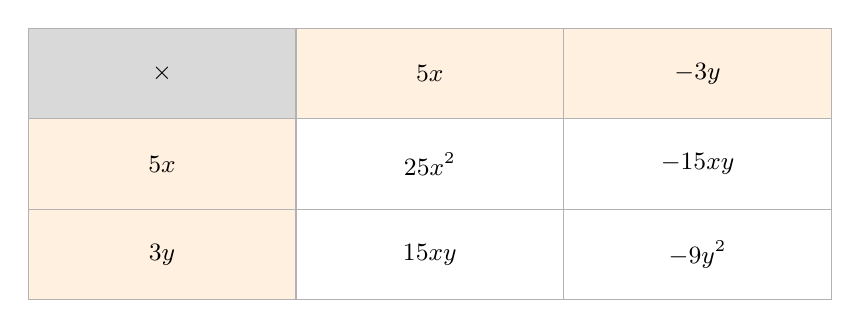
\begin{tikzpicture}[x=1cm,y=1cm,every node/.style={font=\small}]
\fill[gray!30] (0,0) rectangle (3.4,-1.15);
\draw[gray!60] (0,0) rectangle (3.4,-1.15);
\node at (1.7,-0.575) {$\displaystyle \times$};
\fill[orange!12] (3.4,0) rectangle (6.8,-1.15);
\draw[gray!60] (3.4,0) rectangle (6.8,-1.15);
\node at (5.1,-0.575) {$\displaystyle 5x$};
\fill[orange!12] (6.8,0) rectangle (10.2,-1.15);
\draw[gray!60] (6.8,0) rectangle (10.2,-1.15);
\node at (8.5,-0.575) {$\displaystyle -3y$};
\fill[orange!12] (0,-1.15) rectangle (3.4,-2.3);
\draw[gray!60] (0,-1.15) rectangle (3.4,-2.3);
\node at (1.7,-1.725) {$\displaystyle 5x$};
\fill[white] (3.4,-1.15) rectangle (6.8,-2.3);
\draw[gray!60] (3.4,-1.15) rectangle (6.8,-2.3);
\node at (5.1,-1.725) {$\displaystyle 25x^2$};
\fill[white] (6.8,-1.15) rectangle (10.2,-2.3);
\draw[gray!60] (6.8,-1.15) rectangle (10.2,-2.3);
\node at (8.5,-1.725) {$\displaystyle -15xy$};
\fill[orange!12] (0,-2.3) rectangle (3.4,-3.45);
\draw[gray!60] (0,-2.3) rectangle (3.4,-3.45);
\node at (1.7,-2.875) {$\displaystyle 3y$};
\fill[white] (3.4,-2.3) rectangle (6.8,-3.45);
\draw[gray!60] (3.4,-2.3) rectangle (6.8,-3.45);
\node at (5.1,-2.875) {$\displaystyle 15xy$};
\fill[white] (6.8,-2.3) rectangle (10.2,-3.45);
\draw[gray!60] (6.8,-2.3) rectangle (10.2,-3.45);
\node at (8.5,-2.875) {$\displaystyle -9y^2$};
\end{tikzpicture}
\end{center}
\small Take out the common factor $2$ first, then this grid factorises $25x^2-9y^2$ (DOTS).\normalsize

\medskip\hrule

\section*{Factorising 6\quad\small\texttt{(a2-006)}}
\addcontentsline{toc}{section}{Factorising 6 (a2-006)}
\textit{Difficulty: Foundation \quad\textbar\quad Marks: 2}

\question{Write the expression as a product of factors: \( m^2 - 7 \)}

\textbf{Worked solution.}

\textit{Treat 7 as the square of a surd, \( (\sqrt{7})^2 \), to apply the difference of two squares.}
\[\begin{gathered}
m^2 - (\sqrt{7})^2
\end{gathered}\]
Set up the difference of two squares using a square root.

\begin{answerbox}
\textbf{Final answer:}\quad \(\displaystyle (m - \sqrt{7})(m + \sqrt{7})\)
\end{answerbox}
\textbf{Area-model diagram.}

\begin{center}
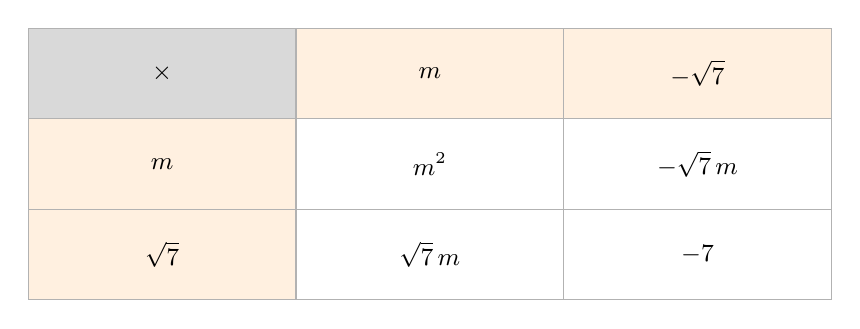
\begin{tikzpicture}[x=1cm,y=1cm,every node/.style={font=\small}]
\fill[gray!30] (0,0) rectangle (3.4,-1.15);
\draw[gray!60] (0,0) rectangle (3.4,-1.15);
\node at (1.7,-0.575) {$\displaystyle \times$};
\fill[orange!12] (3.4,0) rectangle (6.8,-1.15);
\draw[gray!60] (3.4,0) rectangle (6.8,-1.15);
\node at (5.1,-0.575) {$\displaystyle m$};
\fill[orange!12] (6.8,0) rectangle (10.2,-1.15);
\draw[gray!60] (6.8,0) rectangle (10.2,-1.15);
\node at (8.5,-0.575) {$\displaystyle -\sqrt{7}$};
\fill[orange!12] (0,-1.15) rectangle (3.4,-2.3);
\draw[gray!60] (0,-1.15) rectangle (3.4,-2.3);
\node at (1.7,-1.725) {$\displaystyle m$};
\fill[white] (3.4,-1.15) rectangle (6.8,-2.3);
\draw[gray!60] (3.4,-1.15) rectangle (6.8,-2.3);
\node at (5.1,-1.725) {$\displaystyle m^2$};
\fill[white] (6.8,-1.15) rectangle (10.2,-2.3);
\draw[gray!60] (6.8,-1.15) rectangle (10.2,-2.3);
\node at (8.5,-1.725) {$\displaystyle -\sqrt{7}\,m$};
\fill[orange!12] (0,-2.3) rectangle (3.4,-3.45);
\draw[gray!60] (0,-2.3) rectangle (3.4,-3.45);
\node at (1.7,-2.875) {$\displaystyle \sqrt{7}$};
\fill[white] (3.4,-2.3) rectangle (6.8,-3.45);
\draw[gray!60] (3.4,-2.3) rectangle (6.8,-3.45);
\node at (5.1,-2.875) {$\displaystyle \sqrt{7}\,m$};
\fill[white] (6.8,-2.3) rectangle (10.2,-3.45);
\draw[gray!60] (6.8,-2.3) rectangle (10.2,-3.45);
\node at (8.5,-2.875) {$\displaystyle -7$};
\end{tikzpicture}
\end{center}
\small Treat $7$ as $(\sqrt{7})^2$; the cross terms cancel.\normalsize

\medskip\hrule

\section*{Factorising 7\quad\small\texttt{(a2-007)}}
\addcontentsline{toc}{section}{Factorising 7 (a2-007)}
\textit{Difficulty: Foundation \quad\textbar\quad Marks: 2}

\question{Express as the product of factors: \( (x+y)^2 + 5(x+y) \)}

\textbf{Worked solution.}

\textit{Notice that the binomial \( (x+y) \) is a common factor in both parts of the expression.}
\[\begin{gathered}
(x+y)[(x+y) + 5]
\end{gathered}\]
Extract the common bracket.

\begin{answerbox}
\textbf{Final answer:}\quad \(\displaystyle (x+y)(x+y+5)\)
\end{answerbox}
\textbf{Area-model diagram.}

\begin{center}
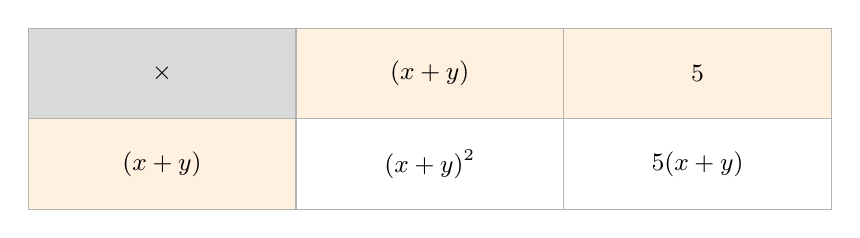
\begin{tikzpicture}[x=1cm,y=1cm,every node/.style={font=\small}]
\fill[gray!30] (0,0) rectangle (3.4,-1.15);
\draw[gray!60] (0,0) rectangle (3.4,-1.15);
\node at (1.7,-0.575) {$\displaystyle \times$};
\fill[orange!12] (3.4,0) rectangle (6.8,-1.15);
\draw[gray!60] (3.4,0) rectangle (6.8,-1.15);
\node at (5.1,-0.575) {$\displaystyle (x+y)$};
\fill[orange!12] (6.8,0) rectangle (10.2,-1.15);
\draw[gray!60] (6.8,0) rectangle (10.2,-1.15);
\node at (8.5,-0.575) {$\displaystyle 5$};
\fill[orange!12] (0,-1.15) rectangle (3.4,-2.3);
\draw[gray!60] (0,-1.15) rectangle (3.4,-2.3);
\node at (1.7,-1.725) {$\displaystyle (x+y)$};
\fill[white] (3.4,-1.15) rectangle (6.8,-2.3);
\draw[gray!60] (3.4,-1.15) rectangle (6.8,-2.3);
\node at (5.1,-1.725) {$\displaystyle (x+y)^2$};
\fill[white] (6.8,-1.15) rectangle (10.2,-2.3);
\draw[gray!60] (6.8,-1.15) rectangle (10.2,-2.3);
\node at (8.5,-1.725) {$\displaystyle 5(x+y)$};
\end{tikzpicture}
\end{center}
\small The whole bracket $(x+y)$ is the common factor.\normalsize

\medskip\hrule

\section*{Factorising 8\quad\small\texttt{(a2-008)}}
\addcontentsline{toc}{section}{Factorising 8 (a2-008)}
\textit{Difficulty: Foundation \quad\textbar\quad Marks: 3}

\question{Express as the product of factors: \( a^2(b-3c) + 4d(3c-b) \)}

\textbf{Worked solution.}

\textit{Step 1: The brackets \( (b-3c) \) and \( (3c-b) \) are opposites. Factor out -1 from the second term to make them match.}
\[\begin{gathered}
a^2(b-3c) - 4d(b-3c)
\end{gathered}\]
Reverse the sign to reveal a common bracket.

\textit{Step 2: Factor out the newly found common bracket.}
\[\begin{gathered}
(b-3c)(a^2-4d)
\end{gathered}\]
Extract the common binomial factor.

\begin{answerbox}
\textbf{Final answer:}\quad \(\displaystyle (b-3c)(a^2-4d)\)
\end{answerbox}
\textbf{Area-model diagram.}

\begin{center}
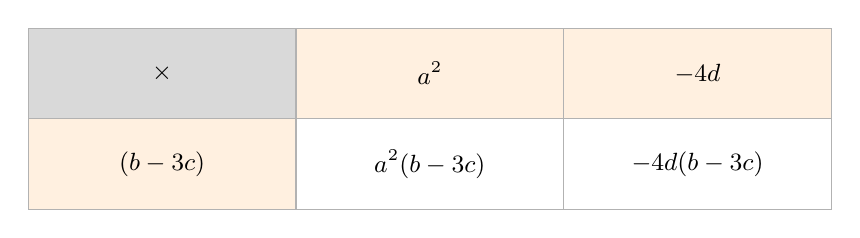
\begin{tikzpicture}[x=1cm,y=1cm,every node/.style={font=\small}]
\fill[gray!30] (0,0) rectangle (3.4,-1.15);
\draw[gray!60] (0,0) rectangle (3.4,-1.15);
\node at (1.7,-0.575) {$\displaystyle \times$};
\fill[orange!12] (3.4,0) rectangle (6.8,-1.15);
\draw[gray!60] (3.4,0) rectangle (6.8,-1.15);
\node at (5.1,-0.575) {$\displaystyle a^2$};
\fill[orange!12] (6.8,0) rectangle (10.2,-1.15);
\draw[gray!60] (6.8,0) rectangle (10.2,-1.15);
\node at (8.5,-0.575) {$\displaystyle -4d$};
\fill[orange!12] (0,-1.15) rectangle (3.4,-2.3);
\draw[gray!60] (0,-1.15) rectangle (3.4,-2.3);
\node at (1.7,-1.725) {$\displaystyle (b-3c)$};
\fill[white] (3.4,-1.15) rectangle (6.8,-2.3);
\draw[gray!60] (3.4,-1.15) rectangle (6.8,-2.3);
\node at (5.1,-1.725) {$\displaystyle a^2(b-3c)$};
\fill[white] (6.8,-1.15) rectangle (10.2,-2.3);
\draw[gray!60] (6.8,-1.15) rectangle (10.2,-2.3);
\node at (8.5,-1.725) {$\displaystyle -4d(b-3c)$};
\end{tikzpicture}
\end{center}
\small Rewrite $4d(3c-b)=-4d(b-3c)$ so both terms share $(b-3c)$.\normalsize

\medskip\hrule

\section*{Factorising 9\quad\small\texttt{(a2-009)}}
\addcontentsline{toc}{section}{Factorising 9 (a2-009)}
\textit{Difficulty: Foundation \quad\textbar\quad Marks: 3}

\question{Simplify the expression, leaving your answer in factorised form: \( 3(m-n)^2 - 6m(m-n) \)}

\textbf{Worked solution.}

\textit{Step 1: Identify and factor out the common factor of \( 3(m-n) \).}
\[\begin{gathered}
3(m-n)[(m-n) - 2m]
\end{gathered}\]
Extract the shared numerical and binomial factors.

\textit{Step 2: Simplify the expression inside the square brackets: \( m - n - 2m = -m - n \).}
\[\begin{gathered}
3(m-n)(-m-n)
\end{gathered}\]
Collect like terms inside the remaining factor.

\begin{answerbox}
\textbf{Final answer:}\quad \(\displaystyle -3(m-n)(m+n)\)
\end{answerbox}
\textbf{Area-model diagram.}

\begin{center}
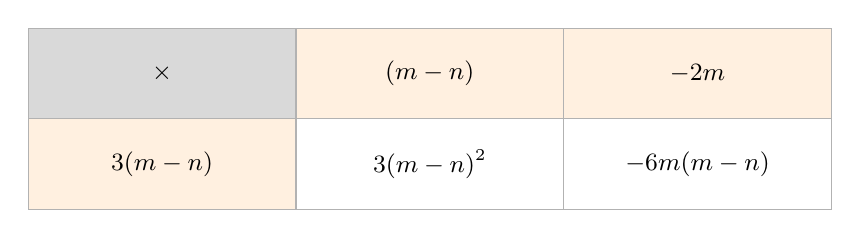
\begin{tikzpicture}[x=1cm,y=1cm,every node/.style={font=\small}]
\fill[gray!30] (0,0) rectangle (3.4,-1.15);
\draw[gray!60] (0,0) rectangle (3.4,-1.15);
\node at (1.7,-0.575) {$\displaystyle \times$};
\fill[orange!12] (3.4,0) rectangle (6.8,-1.15);
\draw[gray!60] (3.4,0) rectangle (6.8,-1.15);
\node at (5.1,-0.575) {$\displaystyle (m-n)$};
\fill[orange!12] (6.8,0) rectangle (10.2,-1.15);
\draw[gray!60] (6.8,0) rectangle (10.2,-1.15);
\node at (8.5,-0.575) {$\displaystyle -2m$};
\fill[orange!12] (0,-1.15) rectangle (3.4,-2.3);
\draw[gray!60] (0,-1.15) rectangle (3.4,-2.3);
\node at (1.7,-1.725) {$\displaystyle 3(m-n)$};
\fill[white] (3.4,-1.15) rectangle (6.8,-2.3);
\draw[gray!60] (3.4,-1.15) rectangle (6.8,-2.3);
\node at (5.1,-1.725) {$\displaystyle 3(m-n)^2$};
\fill[white] (6.8,-1.15) rectangle (10.2,-2.3);
\draw[gray!60] (6.8,-1.15) rectangle (10.2,-2.3);
\node at (8.5,-1.725) {$\displaystyle -6m(m-n)$};
\end{tikzpicture}
\end{center}
\small Common factor $3(m-n)$; then $(m-n)-2m=-(m+n)$ gives $-3(m-n)(m+n)$.\normalsize

\medskip\hrule

\section*{Factorising 10\quad\small\texttt{(a2-010)}}
\addcontentsline{toc}{section}{Factorising 10 (a2-010)}
\textit{Difficulty: Foundation \quad\textbar\quad Marks: 3}

\question{Factorise fully: \( (p+2q)^2 + p + 2q \)}

\textbf{Worked solution.}

\textit{Step 1: Group the last two terms together to reveal a hidden common binomial factor.}
\[\begin{gathered}
(p+2q)^2 + 1(p+2q)
\end{gathered}\]
Recognise that \( p + 2q \) is identical to the expression inside the squared bracket.

\textit{Step 2: Factor out the common bracket \( (p+2q) \).}
\[\begin{gathered}
(p+2q)[(p+2q) + 1]
\end{gathered}\]
Extract the shared factor from both parts of the expression.

\begin{answerbox}
\textbf{Final answer:}\quad \(\displaystyle (p+2q)(p+2q+1)\)
\end{answerbox}
\textbf{Area-model diagram.}

\begin{center}
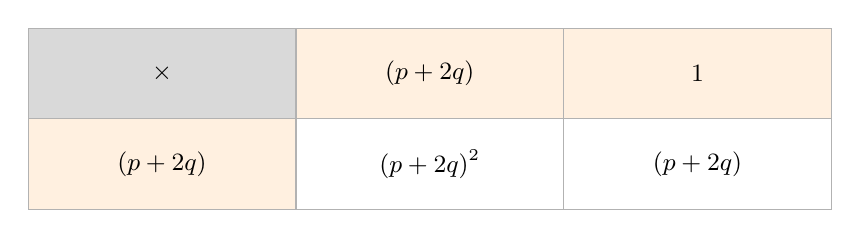
\begin{tikzpicture}[x=1cm,y=1cm,every node/.style={font=\small}]
\fill[gray!30] (0,0) rectangle (3.4,-1.15);
\draw[gray!60] (0,0) rectangle (3.4,-1.15);
\node at (1.7,-0.575) {$\displaystyle \times$};
\fill[orange!12] (3.4,0) rectangle (6.8,-1.15);
\draw[gray!60] (3.4,0) rectangle (6.8,-1.15);
\node at (5.1,-0.575) {$\displaystyle (p+2q)$};
\fill[orange!12] (6.8,0) rectangle (10.2,-1.15);
\draw[gray!60] (6.8,0) rectangle (10.2,-1.15);
\node at (8.5,-0.575) {$\displaystyle 1$};
\fill[orange!12] (0,-1.15) rectangle (3.4,-2.3);
\draw[gray!60] (0,-1.15) rectangle (3.4,-2.3);
\node at (1.7,-1.725) {$\displaystyle (p+2q)$};
\fill[white] (3.4,-1.15) rectangle (6.8,-2.3);
\draw[gray!60] (3.4,-1.15) rectangle (6.8,-2.3);
\node at (5.1,-1.725) {$\displaystyle (p+2q)^2$};
\fill[white] (6.8,-1.15) rectangle (10.2,-2.3);
\draw[gray!60] (6.8,-1.15) rectangle (10.2,-2.3);
\node at (8.5,-1.725) {$\displaystyle (p+2q)$};
\end{tikzpicture}
\end{center}
\small Common bracket $(p+2q)$; the second term contributes a $+1$.\normalsize

\medskip\hrule

\section*{Factorising 11\quad\small\texttt{(a2-011)}}
\addcontentsline{toc}{section}{Factorising 11 (a2-011)}
\textit{Difficulty: Foundation \quad\textbar\quad Marks: 3}

\question{Factorise completely: \( (x+3)^2 - 25 \)}

\textbf{Worked solution.}

\textit{Step 1: Recognise this is a difference of two squares, where \( 25 \) is \( 5^2 \) and \( A = (x+3) \).}
\[\begin{gathered}
[(x+3) - 5][(x+3) + 5]
\end{gathered}\]
Apply the pattern \( A^2 - B^2 = (A-B)(A+B) \).

\textit{Step 2: Simplify the expressions inside each of the new brackets.}
\[\begin{gathered}
(x - 2)(x + 8)
\end{gathered}\]
Collect the number terms together.

\begin{answerbox}
\textbf{Final answer:}\quad \(\displaystyle (x - 2)(x + 8)\)
\end{answerbox}
\textbf{Area-model diagram.}

\begin{center}
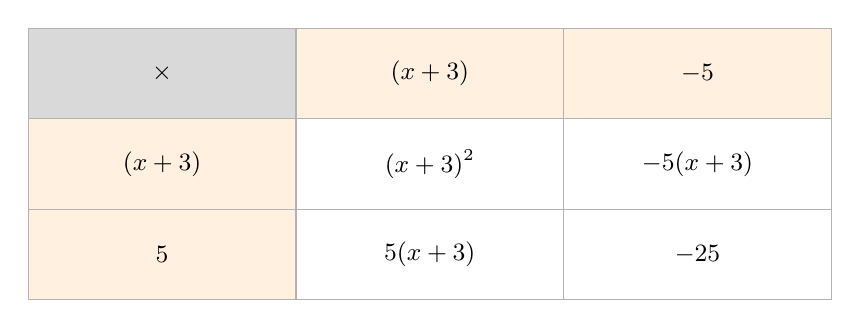
\begin{tikzpicture}[x=1cm,y=1cm,every node/.style={font=\small}]
\fill[gray!30] (0,0) rectangle (3.4,-1.15);
\draw[gray!60] (0,0) rectangle (3.4,-1.15);
\node at (1.7,-0.575) {$\displaystyle \times$};
\fill[orange!12] (3.4,0) rectangle (6.8,-1.15);
\draw[gray!60] (3.4,0) rectangle (6.8,-1.15);
\node at (5.1,-0.575) {$\displaystyle (x+3)$};
\fill[orange!12] (6.8,0) rectangle (10.2,-1.15);
\draw[gray!60] (6.8,0) rectangle (10.2,-1.15);
\node at (8.5,-0.575) {$\displaystyle -5$};
\fill[orange!12] (0,-1.15) rectangle (3.4,-2.3);
\draw[gray!60] (0,-1.15) rectangle (3.4,-2.3);
\node at (1.7,-1.725) {$\displaystyle (x+3)$};
\fill[white] (3.4,-1.15) rectangle (6.8,-2.3);
\draw[gray!60] (3.4,-1.15) rectangle (6.8,-2.3);
\node at (5.1,-1.725) {$\displaystyle (x+3)^2$};
\fill[white] (6.8,-1.15) rectangle (10.2,-2.3);
\draw[gray!60] (6.8,-1.15) rectangle (10.2,-2.3);
\node at (8.5,-1.725) {$\displaystyle -5(x+3)$};
\fill[orange!12] (0,-2.3) rectangle (3.4,-3.45);
\draw[gray!60] (0,-2.3) rectangle (3.4,-3.45);
\node at (1.7,-2.875) {$\displaystyle 5$};
\fill[white] (3.4,-2.3) rectangle (6.8,-3.45);
\draw[gray!60] (3.4,-2.3) rectangle (6.8,-3.45);
\node at (5.1,-2.875) {$\displaystyle 5(x+3)$};
\fill[white] (6.8,-2.3) rectangle (10.2,-3.45);
\draw[gray!60] (6.8,-2.3) rectangle (10.2,-3.45);
\node at (8.5,-2.875) {$\displaystyle -25$};
\end{tikzpicture}
\end{center}
\small DOTS with $a=(x+3),\ b=5$: $(x+3-5)(x+3+5)=(x-2)(x+8)$.\normalsize

\medskip\hrule

\section*{Factorising 12\quad\small\texttt{(a2-012)}}
\addcontentsline{toc}{section}{Factorising 12 (a2-012)}
\textit{Difficulty: Foundation \quad\textbar\quad Marks: 2}

\question{Factorise by grouping: \( ac + ad + bc + bd \)}

\textbf{Worked solution.}

\textit{Step 1: Split the expression in half and factorise the first two terms and the last two terms separately.}
\[\begin{gathered}
a(c+d) + b(c+d)
\end{gathered}\]
Extract the common factor \( a \) from the first pair, and \( b \) from the second pair.

\textit{Step 2: Factor out the newly formed common bracket \( (c+d) \).}
\[\begin{gathered}
(c+d)(a+b)
\end{gathered}\]
Combine the factored groups.

\begin{answerbox}
\textbf{Final answer:}\quad \(\displaystyle (c+d)(a+b)\)
\end{answerbox}
\textbf{Area-model diagram.}

\begin{center}
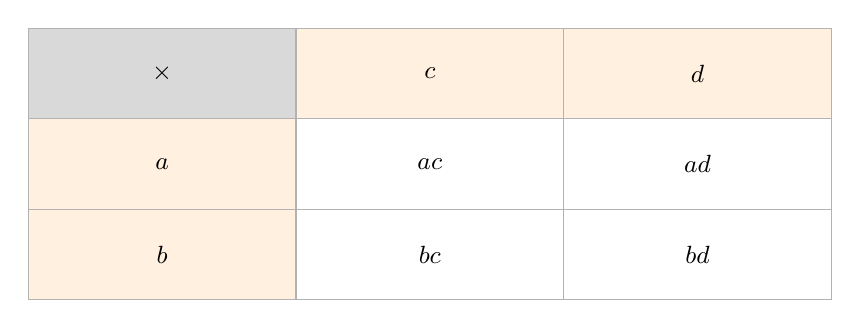
\begin{tikzpicture}[x=1cm,y=1cm,every node/.style={font=\small}]
\fill[gray!30] (0,0) rectangle (3.4,-1.15);
\draw[gray!60] (0,0) rectangle (3.4,-1.15);
\node at (1.7,-0.575) {$\displaystyle \times$};
\fill[orange!12] (3.4,0) rectangle (6.8,-1.15);
\draw[gray!60] (3.4,0) rectangle (6.8,-1.15);
\node at (5.1,-0.575) {$\displaystyle c$};
\fill[orange!12] (6.8,0) rectangle (10.2,-1.15);
\draw[gray!60] (6.8,0) rectangle (10.2,-1.15);
\node at (8.5,-0.575) {$\displaystyle d$};
\fill[orange!12] (0,-1.15) rectangle (3.4,-2.3);
\draw[gray!60] (0,-1.15) rectangle (3.4,-2.3);
\node at (1.7,-1.725) {$\displaystyle a$};
\fill[white] (3.4,-1.15) rectangle (6.8,-2.3);
\draw[gray!60] (3.4,-1.15) rectangle (6.8,-2.3);
\node at (5.1,-1.725) {$\displaystyle ac$};
\fill[white] (6.8,-1.15) rectangle (10.2,-2.3);
\draw[gray!60] (6.8,-1.15) rectangle (10.2,-2.3);
\node at (8.5,-1.725) {$\displaystyle ad$};
\fill[orange!12] (0,-2.3) rectangle (3.4,-3.45);
\draw[gray!60] (0,-2.3) rectangle (3.4,-3.45);
\node at (1.7,-2.875) {$\displaystyle b$};
\fill[white] (3.4,-2.3) rectangle (6.8,-3.45);
\draw[gray!60] (3.4,-2.3) rectangle (6.8,-3.45);
\node at (5.1,-2.875) {$\displaystyle bc$};
\fill[white] (6.8,-2.3) rectangle (10.2,-3.45);
\draw[gray!60] (6.8,-2.3) rectangle (10.2,-3.45);
\node at (8.5,-2.875) {$\displaystyle bd$};
\end{tikzpicture}
\end{center}
\small Grouping: the four given terms are exactly the four cells; read $(a+b)(c+d)$ off the edges.\normalsize

\medskip\hrule

\section*{Factorising 13\quad\small\texttt{(a2-013)}}
\addcontentsline{toc}{section}{Factorising 13 (a2-013)}
\textit{Difficulty: Challenge \quad\textbar\quad Marks: 3}

\question{Simplify the expression, leaving your answer in factorised form: \( (l+w+h)^2 - l(l+w+h) \)}

\textbf{Worked solution.}

\textit{Step 1: Identify \( (l+w+h) \) as a common factor in both terms and extract it.}
\[\begin{gathered}
(l+w+h)[(l+w+h) - l]
\end{gathered}\]
Pull the shared bracket out to the front.

\textit{Step 2: Simplify the expression inside the square brackets: \( l + w + h - l = w + h \).}
\[\begin{gathered}
(l+w+h)(w+h)
\end{gathered}\]
Cancel out the \( l \) and \( -l \).

\begin{answerbox}
\textbf{Final answer:}\quad \(\displaystyle (l+w+h)(w+h)\)
\end{answerbox}
\textbf{Area-model diagram.}

\begin{center}
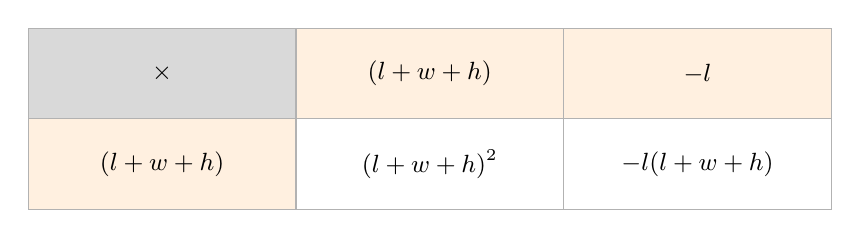
\begin{tikzpicture}[x=1cm,y=1cm,every node/.style={font=\small}]
\fill[gray!30] (0,0) rectangle (3.4,-1.15);
\draw[gray!60] (0,0) rectangle (3.4,-1.15);
\node at (1.7,-0.575) {$\displaystyle \times$};
\fill[orange!12] (3.4,0) rectangle (6.8,-1.15);
\draw[gray!60] (3.4,0) rectangle (6.8,-1.15);
\node at (5.1,-0.575) {$\displaystyle (l+w+h)$};
\fill[orange!12] (6.8,0) rectangle (10.2,-1.15);
\draw[gray!60] (6.8,0) rectangle (10.2,-1.15);
\node at (8.5,-0.575) {$\displaystyle -l$};
\fill[orange!12] (0,-1.15) rectangle (3.4,-2.3);
\draw[gray!60] (0,-1.15) rectangle (3.4,-2.3);
\node at (1.7,-1.725) {$\displaystyle (l+w+h)$};
\fill[white] (3.4,-1.15) rectangle (6.8,-2.3);
\draw[gray!60] (3.4,-1.15) rectangle (6.8,-2.3);
\node at (5.1,-1.725) {$\displaystyle (l+w+h)^2$};
\fill[white] (6.8,-1.15) rectangle (10.2,-2.3);
\draw[gray!60] (6.8,-1.15) rectangle (10.2,-2.3);
\node at (8.5,-1.725) {$\displaystyle -l(l+w+h)$};
\end{tikzpicture}
\end{center}
\small Common bracket $(l+w+h)$; then $(l+w+h)-l=(w+h)$.\normalsize

\medskip\hrule

\section*{Factorising 14\quad\small\texttt{(a2-014)}}
\addcontentsline{toc}{section}{Factorising 14 (a2-014)}
\textit{Difficulty: Foundation \quad\textbar\quad Marks: 2}

\question{Factorise completely: \( -4x^2y - 8xy^2 \)}

\textbf{Worked solution.}

\textit{Step 1: Identify the highest common factor, including the negative sign: \( -4xy \).}
\[\begin{gathered}
-4xy
\end{gathered}\]
Both terms share a factor of -4, x, and y.

\textit{Step 2: Divide both original terms by \( -4xy \) to find the contents of the bracket.}
\[\begin{gathered}
-4xy(x + 2y)
\end{gathered}\]
Ensure the signs inside the bracket become positive because a negative was factored out.

\begin{answerbox}
\textbf{Final answer:}\quad \(\displaystyle -4xy(x + 2y)\)
\end{answerbox}
\textbf{Area-model diagram.}

\begin{center}
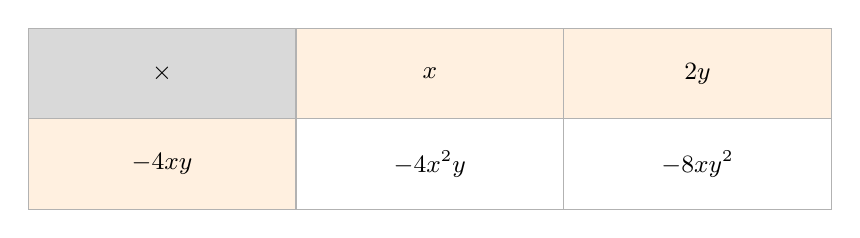
\begin{tikzpicture}[x=1cm,y=1cm,every node/.style={font=\small}]
\fill[gray!30] (0,0) rectangle (3.4,-1.15);
\draw[gray!60] (0,0) rectangle (3.4,-1.15);
\node at (1.7,-0.575) {$\displaystyle \times$};
\fill[orange!12] (3.4,0) rectangle (6.8,-1.15);
\draw[gray!60] (3.4,0) rectangle (6.8,-1.15);
\node at (5.1,-0.575) {$\displaystyle x$};
\fill[orange!12] (6.8,0) rectangle (10.2,-1.15);
\draw[gray!60] (6.8,0) rectangle (10.2,-1.15);
\node at (8.5,-0.575) {$\displaystyle 2y$};
\fill[orange!12] (0,-1.15) rectangle (3.4,-2.3);
\draw[gray!60] (0,-1.15) rectangle (3.4,-2.3);
\node at (1.7,-1.725) {$\displaystyle -4xy$};
\fill[white] (3.4,-1.15) rectangle (6.8,-2.3);
\draw[gray!60] (3.4,-1.15) rectangle (6.8,-2.3);
\node at (5.1,-1.725) {$\displaystyle -4x^2y$};
\fill[white] (6.8,-1.15) rectangle (10.2,-2.3);
\draw[gray!60] (6.8,-1.15) rectangle (10.2,-2.3);
\node at (8.5,-1.725) {$\displaystyle -8xy^2$};
\end{tikzpicture}
\end{center}
\small Take out $-4xy$ (negative HCF) so the bracket starts with $+x$.\normalsize

\medskip\hrule

\section*{Factorising 15\quad\small\texttt{(a2-015)}}
\addcontentsline{toc}{section}{Factorising 15 (a2-015)}
\textit{Difficulty: Foundation \quad\textbar\quad Marks: 4}

\question{Factorise fully: \( 16a^4 - b^4 \)}

\textbf{Worked solution.}

\textit{Step 1: Treat this as a difference of two squares, where the terms are \( (4a^2)^2 \) and \( (b^2)^2 \).}
\[\begin{gathered}
(4a^2 - b^2)(4a^2 + b^2)
\end{gathered}\]
Apply the standard difference of two squares rule to the power of 4 terms.

\textit{Step 2: Recognise that the first bracket, \( (4a^2 - b^2) \), is another difference of two squares.}
\[\begin{gathered}
(2a - b)(2a + b)(4a^2 + b^2)
\end{gathered}\]
Factorise the resulting quadratic, leaving the sum of squares \( (4a^2 + b^2) \) as it cannot be factorised further.

\begin{answerbox}
\textbf{Final answer:}\quad \(\displaystyle (2a - b)(2a + b)(4a^2 + b^2)\)
\end{answerbox}
\textbf{Area-model diagram.}

\begin{center}
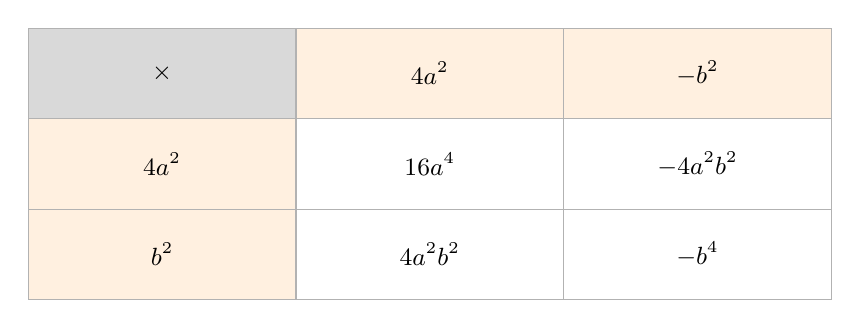
\begin{tikzpicture}[x=1cm,y=1cm,every node/.style={font=\small}]
\fill[gray!30] (0,0) rectangle (3.4,-1.15);
\draw[gray!60] (0,0) rectangle (3.4,-1.15);
\node at (1.7,-0.575) {$\displaystyle \times$};
\fill[orange!12] (3.4,0) rectangle (6.8,-1.15);
\draw[gray!60] (3.4,0) rectangle (6.8,-1.15);
\node at (5.1,-0.575) {$\displaystyle 4a^2$};
\fill[orange!12] (6.8,0) rectangle (10.2,-1.15);
\draw[gray!60] (6.8,0) rectangle (10.2,-1.15);
\node at (8.5,-0.575) {$\displaystyle -b^2$};
\fill[orange!12] (0,-1.15) rectangle (3.4,-2.3);
\draw[gray!60] (0,-1.15) rectangle (3.4,-2.3);
\node at (1.7,-1.725) {$\displaystyle 4a^2$};
\fill[white] (3.4,-1.15) rectangle (6.8,-2.3);
\draw[gray!60] (3.4,-1.15) rectangle (6.8,-2.3);
\node at (5.1,-1.725) {$\displaystyle 16a^4$};
\fill[white] (6.8,-1.15) rectangle (10.2,-2.3);
\draw[gray!60] (6.8,-1.15) rectangle (10.2,-2.3);
\node at (8.5,-1.725) {$\displaystyle -4a^2b^2$};
\fill[orange!12] (0,-2.3) rectangle (3.4,-3.45);
\draw[gray!60] (0,-2.3) rectangle (3.4,-3.45);
\node at (1.7,-2.875) {$\displaystyle b^2$};
\fill[white] (3.4,-2.3) rectangle (6.8,-3.45);
\draw[gray!60] (3.4,-2.3) rectangle (6.8,-3.45);
\node at (5.1,-2.875) {$\displaystyle 4a^2b^2$};
\fill[white] (6.8,-2.3) rectangle (10.2,-3.45);
\draw[gray!60] (6.8,-2.3) rectangle (10.2,-3.45);
\node at (8.5,-2.875) {$\displaystyle -b^4$};
\end{tikzpicture}
\end{center}
\small First DOTS gives $(4a^2-b^2)(4a^2+b^2)$; then $4a^2-b^2=(2a-b)(2a+b)$ is another DOTS.\normalsize

\medskip\hrule

\section*{Factorising 16\quad\small\texttt{(a2-016)}}
\addcontentsline{toc}{section}{Factorising 16 (a2-016)}
\textit{Difficulty: Foundation \quad\textbar\quad Marks: 4}

\question{Simplify the expression, leaving your answer in factorised form: \( x^2(1-y)^2 + x(2-2y) \)}

\textbf{Worked solution.}

\textit{Step 1: Factorise the second term, \( x(2-2y) \), by extracting a 2 to reveal a common bracket.}
\[\begin{gathered}
x^2(1-y)^2 + 2x(1-y)
\end{gathered}\]
Make the brackets match across both terms.

\textit{Step 2: Identify and factor out the common factor of \( x(1-y) \) from the entire expression.}
\[\begin{gathered}
x(1-y)[x(1-y) + 2]
\end{gathered}\]
Extract the shared algebraic and binomial components.

\textit{Step 3: Expand the inner bracket slightly to neaten the final expression (optional but good practice).}
\[\begin{gathered}
x(1-y)(x - xy + 2)
\end{gathered}\]
Distribute the \( x \) inside the square brackets.

\begin{answerbox}
\textbf{Final answer:}\quad \(\displaystyle x(1-y)(x - xy + 2)\)
\end{answerbox}
\textbf{Area-model diagram.}

\begin{center}
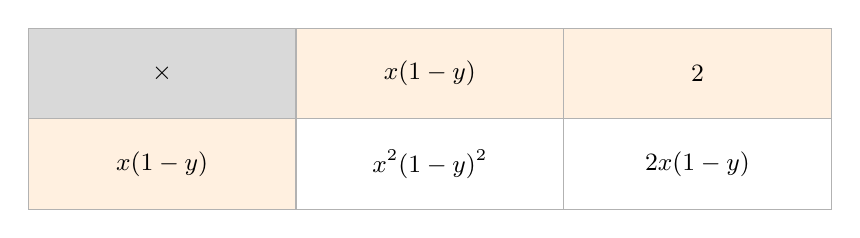
\begin{tikzpicture}[x=1cm,y=1cm,every node/.style={font=\small}]
\fill[gray!30] (0,0) rectangle (3.4,-1.15);
\draw[gray!60] (0,0) rectangle (3.4,-1.15);
\node at (1.7,-0.575) {$\displaystyle \times$};
\fill[orange!12] (3.4,0) rectangle (6.8,-1.15);
\draw[gray!60] (3.4,0) rectangle (6.8,-1.15);
\node at (5.1,-0.575) {$\displaystyle x(1-y)$};
\fill[orange!12] (6.8,0) rectangle (10.2,-1.15);
\draw[gray!60] (6.8,0) rectangle (10.2,-1.15);
\node at (8.5,-0.575) {$\displaystyle 2$};
\fill[orange!12] (0,-1.15) rectangle (3.4,-2.3);
\draw[gray!60] (0,-1.15) rectangle (3.4,-2.3);
\node at (1.7,-1.725) {$\displaystyle x(1-y)$};
\fill[white] (3.4,-1.15) rectangle (6.8,-2.3);
\draw[gray!60] (3.4,-1.15) rectangle (6.8,-2.3);
\node at (5.1,-1.725) {$\displaystyle x^2(1-y)^2$};
\fill[white] (6.8,-1.15) rectangle (10.2,-2.3);
\draw[gray!60] (6.8,-1.15) rectangle (10.2,-2.3);
\node at (8.5,-1.725) {$\displaystyle 2x(1-y)$};
\end{tikzpicture}
\end{center}
\small Since $2-2y=2(1-y)$, the common factor is $x(1-y)$; then $x(1-y)+2=x-xy+2$.\normalsize

\medskip\hrule

\section*{Factorising 17\quad\small\texttt{(a2-017)}}
\addcontentsline{toc}{section}{Factorising 17 (a2-017)}
\textit{Difficulty: Foundation \quad\textbar\quad Marks: 1}

\question{Factorise: \( 15x + 20y \)}

\textbf{Worked solution.}

\textit{Find the highest common factor (HCF) of the numbers 15 and 20, which is 5.}
\[\begin{gathered}
5(3x + 4y)
\end{gathered}\]
Divide both terms by 5 and place the remainder inside the bracket.

\begin{answerbox}
\textbf{Final answer:}\quad \(\displaystyle 5(3x + 4y)\)
\end{answerbox}
\textbf{Area-model diagram.}

\begin{center}
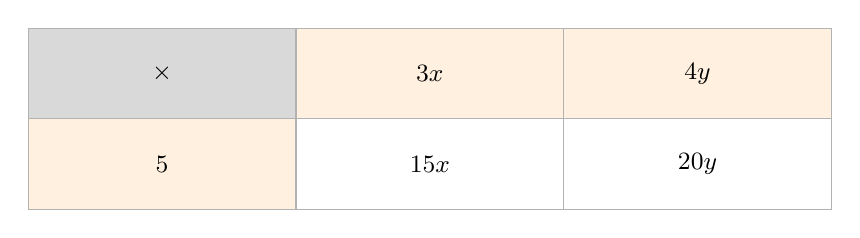
\begin{tikzpicture}[x=1cm,y=1cm,every node/.style={font=\small}]
\fill[gray!30] (0,0) rectangle (3.4,-1.15);
\draw[gray!60] (0,0) rectangle (3.4,-1.15);
\node at (1.7,-0.575) {$\displaystyle \times$};
\fill[orange!12] (3.4,0) rectangle (6.8,-1.15);
\draw[gray!60] (3.4,0) rectangle (6.8,-1.15);
\node at (5.1,-0.575) {$\displaystyle 3x$};
\fill[orange!12] (6.8,0) rectangle (10.2,-1.15);
\draw[gray!60] (6.8,0) rectangle (10.2,-1.15);
\node at (8.5,-0.575) {$\displaystyle 4y$};
\fill[orange!12] (0,-1.15) rectangle (3.4,-2.3);
\draw[gray!60] (0,-1.15) rectangle (3.4,-2.3);
\node at (1.7,-1.725) {$\displaystyle 5$};
\fill[white] (3.4,-1.15) rectangle (6.8,-2.3);
\draw[gray!60] (3.4,-1.15) rectangle (6.8,-2.3);
\node at (5.1,-1.725) {$\displaystyle 15x$};
\fill[white] (6.8,-1.15) rectangle (10.2,-2.3);
\draw[gray!60] (6.8,-1.15) rectangle (10.2,-2.3);
\node at (8.5,-1.725) {$\displaystyle 20y$};
\end{tikzpicture}
\end{center}
\small HCF $5$.\normalsize

\medskip\hrule

\section*{Factorising 18\quad\small\texttt{(a2-018)}}
\addcontentsline{toc}{section}{Factorising 18 (a2-018)}
\textit{Difficulty: Standard \quad\textbar\quad Marks: 2}

\question{Factorise fully: \( 6a^2b - 9ab^2 \)}

\textbf{Worked solution.}

\textit{Step 1: Identify the HCF of 6 and 9 (which is 3) and the common variables (which are \( a \) and \( b \)).}
\[\begin{gathered}
3ab
\end{gathered}\]
Find the highest algebraic and numerical factors shared by both terms.

\textit{Step 2: Factor out \( 3ab \) from the original expression.}
\[\begin{gathered}
3ab(2a - 3b)
\end{gathered}\]
Divide each term by \( 3ab \) to find the expression inside the bracket.

\begin{answerbox}
\textbf{Final answer:}\quad \(\displaystyle 3ab(2a - 3b)\)
\end{answerbox}
\textbf{Area-model diagram.}

\begin{center}
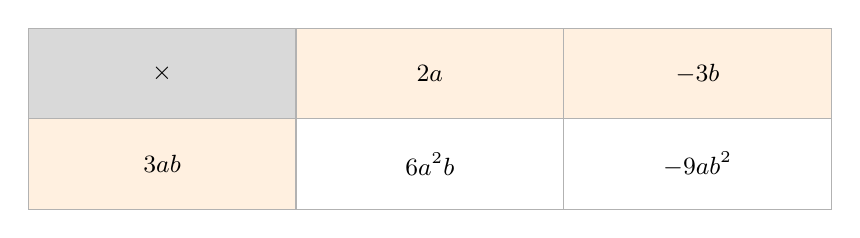
\begin{tikzpicture}[x=1cm,y=1cm,every node/.style={font=\small}]
\fill[gray!30] (0,0) rectangle (3.4,-1.15);
\draw[gray!60] (0,0) rectangle (3.4,-1.15);
\node at (1.7,-0.575) {$\displaystyle \times$};
\fill[orange!12] (3.4,0) rectangle (6.8,-1.15);
\draw[gray!60] (3.4,0) rectangle (6.8,-1.15);
\node at (5.1,-0.575) {$\displaystyle 2a$};
\fill[orange!12] (6.8,0) rectangle (10.2,-1.15);
\draw[gray!60] (6.8,0) rectangle (10.2,-1.15);
\node at (8.5,-0.575) {$\displaystyle -3b$};
\fill[orange!12] (0,-1.15) rectangle (3.4,-2.3);
\draw[gray!60] (0,-1.15) rectangle (3.4,-2.3);
\node at (1.7,-1.725) {$\displaystyle 3ab$};
\fill[white] (3.4,-1.15) rectangle (6.8,-2.3);
\draw[gray!60] (3.4,-1.15) rectangle (6.8,-2.3);
\node at (5.1,-1.725) {$\displaystyle 6a^2b$};
\fill[white] (6.8,-1.15) rectangle (10.2,-2.3);
\draw[gray!60] (6.8,-1.15) rectangle (10.2,-2.3);
\node at (8.5,-1.725) {$\displaystyle -9ab^2$};
\end{tikzpicture}
\end{center}
\small HCF $3ab$.\normalsize

\medskip\hrule

\section*{Factorising 19\quad\small\texttt{(a2-019)}}
\addcontentsline{toc}{section}{Factorising 19 (a2-019)}
\textit{Difficulty: Foundation \quad\textbar\quad Marks: 1}

\question{Write the expression as a product of factors: \( y^2 - 81 \)}

\textbf{Worked solution.}

\textit{Recognise that this is a difference of two squares, where 81 is \( 9^2 \).}
\[\begin{gathered}
y^2 - 9^2
\end{gathered}\]
Identify the squared terms to apply the rule \( A^2 - B^2 = (A-B)(A+B) \).

\begin{answerbox}
\textbf{Final answer:}\quad \(\displaystyle (y - 9)(y + 9)\)
\end{answerbox}
\textbf{Area-model diagram.}

\begin{center}
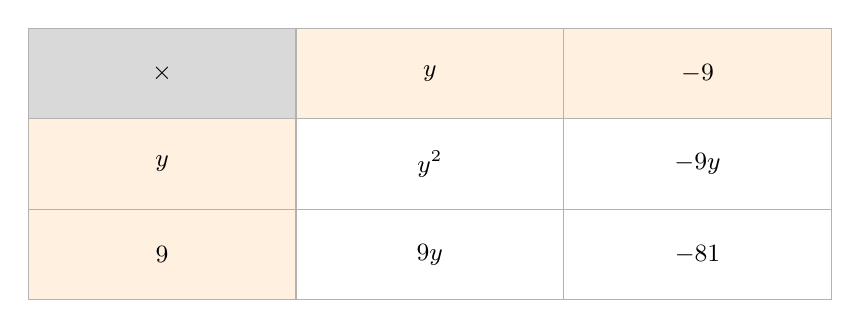
\begin{tikzpicture}[x=1cm,y=1cm,every node/.style={font=\small}]
\fill[gray!30] (0,0) rectangle (3.4,-1.15);
\draw[gray!60] (0,0) rectangle (3.4,-1.15);
\node at (1.7,-0.575) {$\displaystyle \times$};
\fill[orange!12] (3.4,0) rectangle (6.8,-1.15);
\draw[gray!60] (3.4,0) rectangle (6.8,-1.15);
\node at (5.1,-0.575) {$\displaystyle y$};
\fill[orange!12] (6.8,0) rectangle (10.2,-1.15);
\draw[gray!60] (6.8,0) rectangle (10.2,-1.15);
\node at (8.5,-0.575) {$\displaystyle -9$};
\fill[orange!12] (0,-1.15) rectangle (3.4,-2.3);
\draw[gray!60] (0,-1.15) rectangle (3.4,-2.3);
\node at (1.7,-1.725) {$\displaystyle y$};
\fill[white] (3.4,-1.15) rectangle (6.8,-2.3);
\draw[gray!60] (3.4,-1.15) rectangle (6.8,-2.3);
\node at (5.1,-1.725) {$\displaystyle y^2$};
\fill[white] (6.8,-1.15) rectangle (10.2,-2.3);
\draw[gray!60] (6.8,-1.15) rectangle (10.2,-2.3);
\node at (8.5,-1.725) {$\displaystyle -9y$};
\fill[orange!12] (0,-2.3) rectangle (3.4,-3.45);
\draw[gray!60] (0,-2.3) rectangle (3.4,-3.45);
\node at (1.7,-2.875) {$\displaystyle 9$};
\fill[white] (3.4,-2.3) rectangle (6.8,-3.45);
\draw[gray!60] (3.4,-2.3) rectangle (6.8,-3.45);
\node at (5.1,-2.875) {$\displaystyle 9y$};
\fill[white] (6.8,-2.3) rectangle (10.2,-3.45);
\draw[gray!60] (6.8,-2.3) rectangle (10.2,-3.45);
\node at (8.5,-2.875) {$\displaystyle -81$};
\end{tikzpicture}
\end{center}
\small DOTS: $81=9^2$, cross terms cancel.\normalsize

\medskip\hrule

\section*{Factorising 20\quad\small\texttt{(a2-020)}}
\addcontentsline{toc}{section}{Factorising 20 (a2-020)}
\textit{Difficulty: Foundation \quad\textbar\quad Marks: 3}

\question{Factorise completely: \( 3x^2 - 75 \)}

\textbf{Worked solution.}

\textit{Step 1: Extract the common numerical factor of 3 from both terms first.}
\[\begin{gathered}
3(x^2 - 25)
\end{gathered}\]
Always check for a common factor before applying other factorisation rules.

\textit{Step 2: Factorise the expression inside the bracket using the difference of two squares rule.}
\[\begin{gathered}
3(x - 5)(x + 5)
\end{gathered}\]
Recognise that 25 is \( 5^2 \).

\begin{answerbox}
\textbf{Final answer:}\quad \(\displaystyle 3(x - 5)(x + 5)\)
\end{answerbox}
\textbf{Area-model diagram.}

\begin{center}
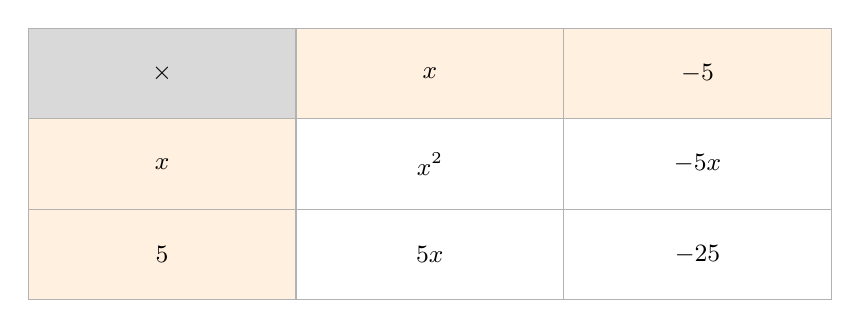
\begin{tikzpicture}[x=1cm,y=1cm,every node/.style={font=\small}]
\fill[gray!30] (0,0) rectangle (3.4,-1.15);
\draw[gray!60] (0,0) rectangle (3.4,-1.15);
\node at (1.7,-0.575) {$\displaystyle \times$};
\fill[orange!12] (3.4,0) rectangle (6.8,-1.15);
\draw[gray!60] (3.4,0) rectangle (6.8,-1.15);
\node at (5.1,-0.575) {$\displaystyle x$};
\fill[orange!12] (6.8,0) rectangle (10.2,-1.15);
\draw[gray!60] (6.8,0) rectangle (10.2,-1.15);
\node at (8.5,-0.575) {$\displaystyle -5$};
\fill[orange!12] (0,-1.15) rectangle (3.4,-2.3);
\draw[gray!60] (0,-1.15) rectangle (3.4,-2.3);
\node at (1.7,-1.725) {$\displaystyle x$};
\fill[white] (3.4,-1.15) rectangle (6.8,-2.3);
\draw[gray!60] (3.4,-1.15) rectangle (6.8,-2.3);
\node at (5.1,-1.725) {$\displaystyle x^2$};
\fill[white] (6.8,-1.15) rectangle (10.2,-2.3);
\draw[gray!60] (6.8,-1.15) rectangle (10.2,-2.3);
\node at (8.5,-1.725) {$\displaystyle -5x$};
\fill[orange!12] (0,-2.3) rectangle (3.4,-3.45);
\draw[gray!60] (0,-2.3) rectangle (3.4,-3.45);
\node at (1.7,-2.875) {$\displaystyle 5$};
\fill[white] (3.4,-2.3) rectangle (6.8,-3.45);
\draw[gray!60] (3.4,-2.3) rectangle (6.8,-3.45);
\node at (5.1,-2.875) {$\displaystyle 5x$};
\fill[white] (6.8,-2.3) rectangle (10.2,-3.45);
\draw[gray!60] (6.8,-2.3) rectangle (10.2,-3.45);
\node at (8.5,-2.875) {$\displaystyle -25$};
\end{tikzpicture}
\end{center}
\small Take out $3$ first: $3(x^2-25)$, then DOTS on $x^2-25$.\normalsize

\medskip\hrule

\section*{Factorising 21\quad\small\texttt{(a2-021)}}
\addcontentsline{toc}{section}{Factorising 21 (a2-021)}
\textit{Difficulty: Foundation \quad\textbar\quad Marks: 2}

\question{Factorise by grouping: \( xy + 2x + 3y + 6 \)}

\textbf{Worked solution.}

\textit{Step 1: Group the first two terms and the last two terms, then factorise them separately.}
\[\begin{gathered}
x(y + 2) + 3(y + 2)
\end{gathered}\]
Extract \( x \) from the first pair and 3 from the second pair.

\textit{Step 2: Factor out the common binomial bracket \( (y + 2) \).}
\[\begin{gathered}
(y + 2)(x + 3)
\end{gathered}\]
Combine the factored groups together.

\begin{answerbox}
\textbf{Final answer:}\quad \(\displaystyle (y + 2)(x + 3)\)
\end{answerbox}
\textbf{Area-model diagram.}

\begin{center}
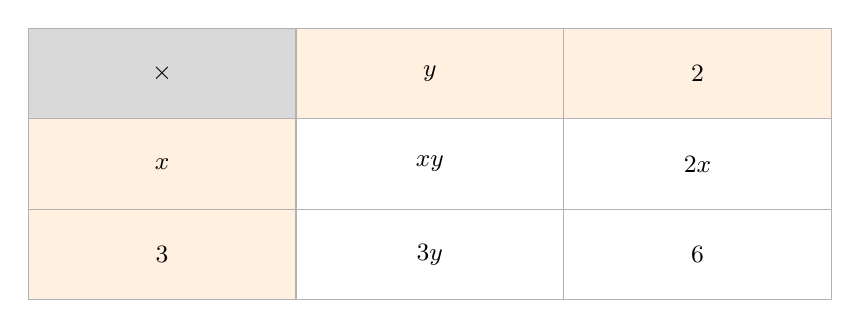
\begin{tikzpicture}[x=1cm,y=1cm,every node/.style={font=\small}]
\fill[gray!30] (0,0) rectangle (3.4,-1.15);
\draw[gray!60] (0,0) rectangle (3.4,-1.15);
\node at (1.7,-0.575) {$\displaystyle \times$};
\fill[orange!12] (3.4,0) rectangle (6.8,-1.15);
\draw[gray!60] (3.4,0) rectangle (6.8,-1.15);
\node at (5.1,-0.575) {$\displaystyle y$};
\fill[orange!12] (6.8,0) rectangle (10.2,-1.15);
\draw[gray!60] (6.8,0) rectangle (10.2,-1.15);
\node at (8.5,-0.575) {$\displaystyle 2$};
\fill[orange!12] (0,-1.15) rectangle (3.4,-2.3);
\draw[gray!60] (0,-1.15) rectangle (3.4,-2.3);
\node at (1.7,-1.725) {$\displaystyle x$};
\fill[white] (3.4,-1.15) rectangle (6.8,-2.3);
\draw[gray!60] (3.4,-1.15) rectangle (6.8,-2.3);
\node at (5.1,-1.725) {$\displaystyle xy$};
\fill[white] (6.8,-1.15) rectangle (10.2,-2.3);
\draw[gray!60] (6.8,-1.15) rectangle (10.2,-2.3);
\node at (8.5,-1.725) {$\displaystyle 2x$};
\fill[orange!12] (0,-2.3) rectangle (3.4,-3.45);
\draw[gray!60] (0,-2.3) rectangle (3.4,-3.45);
\node at (1.7,-2.875) {$\displaystyle 3$};
\fill[white] (3.4,-2.3) rectangle (6.8,-3.45);
\draw[gray!60] (3.4,-2.3) rectangle (6.8,-3.45);
\node at (5.1,-2.875) {$\displaystyle 3y$};
\fill[white] (6.8,-2.3) rectangle (10.2,-3.45);
\draw[gray!60] (6.8,-2.3) rectangle (10.2,-3.45);
\node at (8.5,-2.875) {$\displaystyle 6$};
\end{tikzpicture}
\end{center}
\small Grouping: $x(y+2)+3(y+2)=(x+3)(y+2)$.\normalsize

\medskip\hrule

\section*{Factorising 22\quad\small\texttt{(a2-022)}}
\addcontentsline{toc}{section}{Factorising 22 (a2-022)}
\textit{Difficulty: Foundation \quad\textbar\quad Marks: 2}

\question{Express as a product of factors: \( (a-b)^2 + 2(a-b) \)}

\textbf{Worked solution.}

\textit{Step 1: Identify that the bracket \( (a-b) \) is a common factor in both terms.}
\[\begin{gathered}
(a-b)[(a-b) + 2]
\end{gathered}\]
Extract the shared binomial bracket to the front.

\textit{Step 2: Remove the inner square brackets for the final simplified answer.}
\[\begin{gathered}
(a-b)(a-b+2)
\end{gathered}\]
Neaten up the expression.

\begin{answerbox}
\textbf{Final answer:}\quad \(\displaystyle (a-b)(a-b+2)\)
\end{answerbox}
\textbf{Area-model diagram.}

\begin{center}
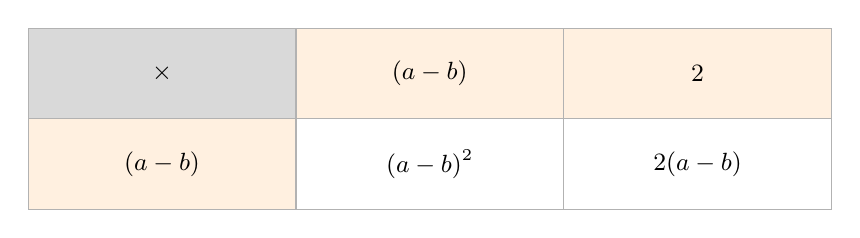
\begin{tikzpicture}[x=1cm,y=1cm,every node/.style={font=\small}]
\fill[gray!30] (0,0) rectangle (3.4,-1.15);
\draw[gray!60] (0,0) rectangle (3.4,-1.15);
\node at (1.7,-0.575) {$\displaystyle \times$};
\fill[orange!12] (3.4,0) rectangle (6.8,-1.15);
\draw[gray!60] (3.4,0) rectangle (6.8,-1.15);
\node at (5.1,-0.575) {$\displaystyle (a-b)$};
\fill[orange!12] (6.8,0) rectangle (10.2,-1.15);
\draw[gray!60] (6.8,0) rectangle (10.2,-1.15);
\node at (8.5,-0.575) {$\displaystyle 2$};
\fill[orange!12] (0,-1.15) rectangle (3.4,-2.3);
\draw[gray!60] (0,-1.15) rectangle (3.4,-2.3);
\node at (1.7,-1.725) {$\displaystyle (a-b)$};
\fill[white] (3.4,-1.15) rectangle (6.8,-2.3);
\draw[gray!60] (3.4,-1.15) rectangle (6.8,-2.3);
\node at (5.1,-1.725) {$\displaystyle (a-b)^2$};
\fill[white] (6.8,-1.15) rectangle (10.2,-2.3);
\draw[gray!60] (6.8,-1.15) rectangle (10.2,-2.3);
\node at (8.5,-1.725) {$\displaystyle 2(a-b)$};
\end{tikzpicture}
\end{center}
\small Common bracket $(a-b)$.\normalsize

\medskip\hrule

\section*{Factorising 23\quad\small\texttt{(a2-023)}}
\addcontentsline{toc}{section}{Factorising 23 (a2-023)}
\textit{Difficulty: Foundation \quad\textbar\quad Marks: 3}

\question{Factorise fully: \( 4x^3y - 16xy^3 \)}

\textbf{Worked solution.}

\textit{Step 1: Find and extract the highest common factor for both terms, which is \( 4xy \).}
\[\begin{gathered}
4xy(x^2 - 4y^2)
\end{gathered}\]
Divide both terms by \( 4xy \) to find the remaining expression.

\textit{Step 2: Recognise that the expression inside the bracket is a difference of two squares and factorise it.}
\[\begin{gathered}
4xy(x - 2y)(x + 2y)
\end{gathered}\]
Apply the pattern \( A^2 - B^2 = (A-B)(A+B) \) to \( (x^2 - 4y^2) \).

\begin{answerbox}
\textbf{Final answer:}\quad \(\displaystyle 4xy(x - 2y)(x + 2y)\)
\end{answerbox}
\textbf{Area-model diagram.}

\begin{center}
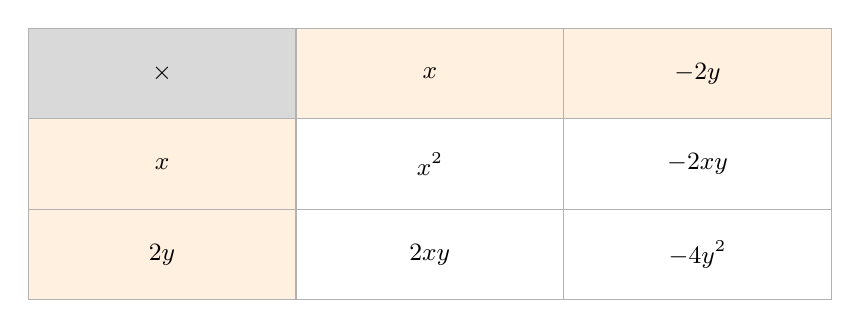
\begin{tikzpicture}[x=1cm,y=1cm,every node/.style={font=\small}]
\fill[gray!30] (0,0) rectangle (3.4,-1.15);
\draw[gray!60] (0,0) rectangle (3.4,-1.15);
\node at (1.7,-0.575) {$\displaystyle \times$};
\fill[orange!12] (3.4,0) rectangle (6.8,-1.15);
\draw[gray!60] (3.4,0) rectangle (6.8,-1.15);
\node at (5.1,-0.575) {$\displaystyle x$};
\fill[orange!12] (6.8,0) rectangle (10.2,-1.15);
\draw[gray!60] (6.8,0) rectangle (10.2,-1.15);
\node at (8.5,-0.575) {$\displaystyle -2y$};
\fill[orange!12] (0,-1.15) rectangle (3.4,-2.3);
\draw[gray!60] (0,-1.15) rectangle (3.4,-2.3);
\node at (1.7,-1.725) {$\displaystyle x$};
\fill[white] (3.4,-1.15) rectangle (6.8,-2.3);
\draw[gray!60] (3.4,-1.15) rectangle (6.8,-2.3);
\node at (5.1,-1.725) {$\displaystyle x^2$};
\fill[white] (6.8,-1.15) rectangle (10.2,-2.3);
\draw[gray!60] (6.8,-1.15) rectangle (10.2,-2.3);
\node at (8.5,-1.725) {$\displaystyle -2xy$};
\fill[orange!12] (0,-2.3) rectangle (3.4,-3.45);
\draw[gray!60] (0,-2.3) rectangle (3.4,-3.45);
\node at (1.7,-2.875) {$\displaystyle 2y$};
\fill[white] (3.4,-2.3) rectangle (6.8,-3.45);
\draw[gray!60] (3.4,-2.3) rectangle (6.8,-3.45);
\node at (5.1,-2.875) {$\displaystyle 2xy$};
\fill[white] (6.8,-2.3) rectangle (10.2,-3.45);
\draw[gray!60] (6.8,-2.3) rectangle (10.2,-3.45);
\node at (8.5,-2.875) {$\displaystyle -4y^2$};
\end{tikzpicture}
\end{center}
\small Take out $4xy$ first: $4xy(x^2-4y^2)$, then DOTS.\normalsize

\medskip\hrule

\section*{Factorising 24\quad\small\texttt{(a2-024)}}
\addcontentsline{toc}{section}{Factorising 24 (a2-024)}
\textit{Difficulty: Foundation \quad\textbar\quad Marks: 1}

\question{Write the expression as a product of factors: \( 100 - z^2 \)}

\textbf{Worked solution.}

\textit{Recognise that this is a difference of two squares, where 100 is \( 10^2 \).}
\[\begin{gathered}
10^2 - z^2
\end{gathered}\]
Identify the squared terms to apply the rule \( A^2 - B^2 = (A-B)(A+B) \).

\begin{answerbox}
\textbf{Final answer:}\quad \(\displaystyle (10 - z)(10 + z)\)
\end{answerbox}
\textbf{Area-model diagram.}

\begin{center}
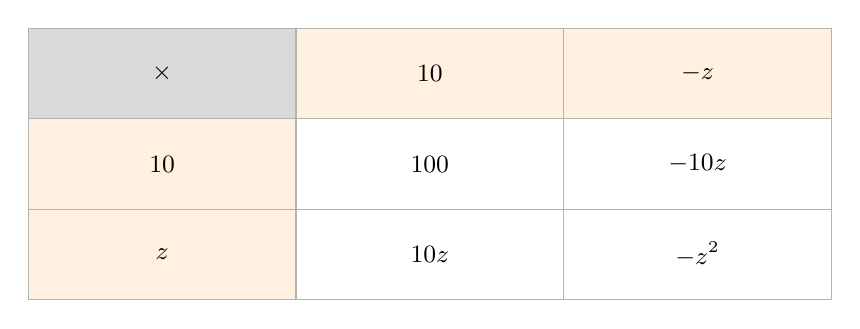
\begin{tikzpicture}[x=1cm,y=1cm,every node/.style={font=\small}]
\fill[gray!30] (0,0) rectangle (3.4,-1.15);
\draw[gray!60] (0,0) rectangle (3.4,-1.15);
\node at (1.7,-0.575) {$\displaystyle \times$};
\fill[orange!12] (3.4,0) rectangle (6.8,-1.15);
\draw[gray!60] (3.4,0) rectangle (6.8,-1.15);
\node at (5.1,-0.575) {$\displaystyle 10$};
\fill[orange!12] (6.8,0) rectangle (10.2,-1.15);
\draw[gray!60] (6.8,0) rectangle (10.2,-1.15);
\node at (8.5,-0.575) {$\displaystyle -z$};
\fill[orange!12] (0,-1.15) rectangle (3.4,-2.3);
\draw[gray!60] (0,-1.15) rectangle (3.4,-2.3);
\node at (1.7,-1.725) {$\displaystyle 10$};
\fill[white] (3.4,-1.15) rectangle (6.8,-2.3);
\draw[gray!60] (3.4,-1.15) rectangle (6.8,-2.3);
\node at (5.1,-1.725) {$\displaystyle 100$};
\fill[white] (6.8,-1.15) rectangle (10.2,-2.3);
\draw[gray!60] (6.8,-1.15) rectangle (10.2,-2.3);
\node at (8.5,-1.725) {$\displaystyle -10z$};
\fill[orange!12] (0,-2.3) rectangle (3.4,-3.45);
\draw[gray!60] (0,-2.3) rectangle (3.4,-3.45);
\node at (1.7,-2.875) {$\displaystyle z$};
\fill[white] (3.4,-2.3) rectangle (6.8,-3.45);
\draw[gray!60] (3.4,-2.3) rectangle (6.8,-3.45);
\node at (5.1,-2.875) {$\displaystyle 10z$};
\fill[white] (6.8,-2.3) rectangle (10.2,-3.45);
\draw[gray!60] (6.8,-2.3) rectangle (10.2,-3.45);
\node at (8.5,-2.875) {$\displaystyle -z^2$};
\end{tikzpicture}
\end{center}
\small DOTS: $100=10^2$.\normalsize

\medskip\hrule

\section*{Factorising 25\quad\small\texttt{(a2-025)}}
\addcontentsline{toc}{section}{Factorising 25 (a2-025)}
\textit{Difficulty: Foundation \quad\textbar\quad Marks: 2}

\question{Factorise completely: \( 14m^2n^3 + 21m^3n^2 \)}

\textbf{Worked solution.}

\textit{Step 1: Identify the highest common factor of the numbers (which is 7) and the highest common powers of the variables (which are \( m^2 \) and \( n^2 \)).}
\[\begin{gathered}
7m^2n^2
\end{gathered}\]
Find the greatest term that divides exactly into both parts of the expression.

\textit{Step 2: Factor out \( 7m^2n^2 \) from the original expression.}
\[\begin{gathered}
7m^2n^2(2n + 3m)
\end{gathered}\]
Divide each term by the common factor to find the contents of the bracket.

\begin{answerbox}
\textbf{Final answer:}\quad \(\displaystyle 7m^2n^2(2n + 3m)\)
\end{answerbox}
\textbf{Area-model diagram.}

\begin{center}
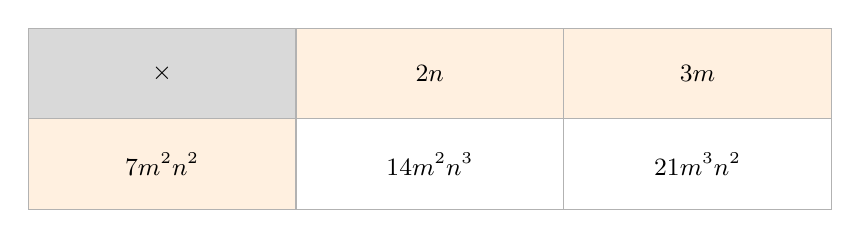
\begin{tikzpicture}[x=1cm,y=1cm,every node/.style={font=\small}]
\fill[gray!30] (0,0) rectangle (3.4,-1.15);
\draw[gray!60] (0,0) rectangle (3.4,-1.15);
\node at (1.7,-0.575) {$\displaystyle \times$};
\fill[orange!12] (3.4,0) rectangle (6.8,-1.15);
\draw[gray!60] (3.4,0) rectangle (6.8,-1.15);
\node at (5.1,-0.575) {$\displaystyle 2n$};
\fill[orange!12] (6.8,0) rectangle (10.2,-1.15);
\draw[gray!60] (6.8,0) rectangle (10.2,-1.15);
\node at (8.5,-0.575) {$\displaystyle 3m$};
\fill[orange!12] (0,-1.15) rectangle (3.4,-2.3);
\draw[gray!60] (0,-1.15) rectangle (3.4,-2.3);
\node at (1.7,-1.725) {$\displaystyle 7m^2n^2$};
\fill[white] (3.4,-1.15) rectangle (6.8,-2.3);
\draw[gray!60] (3.4,-1.15) rectangle (6.8,-2.3);
\node at (5.1,-1.725) {$\displaystyle 14m^2n^3$};
\fill[white] (6.8,-1.15) rectangle (10.2,-2.3);
\draw[gray!60] (6.8,-1.15) rectangle (10.2,-2.3);
\node at (8.5,-1.725) {$\displaystyle 21m^3n^2$};
\end{tikzpicture}
\end{center}
\small HCF $7m^2n^2$.\normalsize

\medskip\hrule

\section*{Factorising 26\quad\small\texttt{(a2-026)}}
\addcontentsline{toc}{section}{Factorising 26 (a2-026)}
\textit{Difficulty: Foundation \quad\textbar\quad Marks: 2}

\question{Express as the product of factors: \( x(x-4) - 3(x-4) \)}

\textbf{Worked solution.}

\textit{Identify that the bracket \( (x-4) \) is a common factor in both terms.}
\[\begin{gathered}
(x-4)(x - 3)
\end{gathered}\]
Extract the shared binomial bracket to the front, placing the remaining outer terms into a second bracket.

\begin{answerbox}
\textbf{Final answer:}\quad \(\displaystyle (x-4)(x-3)\)
\end{answerbox}
\textbf{Area-model diagram.}

\begin{center}
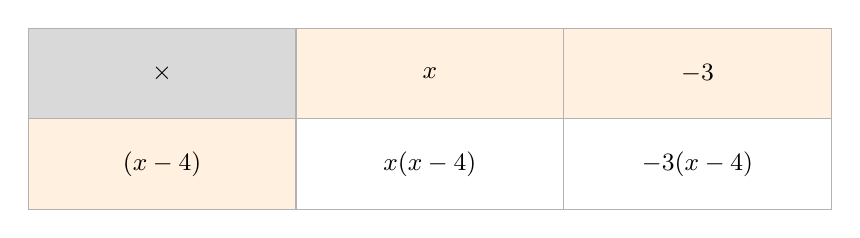
\begin{tikzpicture}[x=1cm,y=1cm,every node/.style={font=\small}]
\fill[gray!30] (0,0) rectangle (3.4,-1.15);
\draw[gray!60] (0,0) rectangle (3.4,-1.15);
\node at (1.7,-0.575) {$\displaystyle \times$};
\fill[orange!12] (3.4,0) rectangle (6.8,-1.15);
\draw[gray!60] (3.4,0) rectangle (6.8,-1.15);
\node at (5.1,-0.575) {$\displaystyle x$};
\fill[orange!12] (6.8,0) rectangle (10.2,-1.15);
\draw[gray!60] (6.8,0) rectangle (10.2,-1.15);
\node at (8.5,-0.575) {$\displaystyle -3$};
\fill[orange!12] (0,-1.15) rectangle (3.4,-2.3);
\draw[gray!60] (0,-1.15) rectangle (3.4,-2.3);
\node at (1.7,-1.725) {$\displaystyle (x-4)$};
\fill[white] (3.4,-1.15) rectangle (6.8,-2.3);
\draw[gray!60] (3.4,-1.15) rectangle (6.8,-2.3);
\node at (5.1,-1.725) {$\displaystyle x(x-4)$};
\fill[white] (6.8,-1.15) rectangle (10.2,-2.3);
\draw[gray!60] (6.8,-1.15) rectangle (10.2,-2.3);
\node at (8.5,-1.725) {$\displaystyle -3(x-4)$};
\end{tikzpicture}
\end{center}
\small Common bracket $(x-4)$; remaining factor $(x-3)$.\normalsize

\medskip\hrule

\section*{Factorising 27\quad\small\texttt{(a2-027)}}
\addcontentsline{toc}{section}{Factorising 27 (a2-027)}
\textit{Difficulty: Foundation \quad\textbar\quad Marks: 3}

\question{Factorise fully: \( 8x^2 - 32y^2 \)}

\textbf{Worked solution.}

\textit{Step 1: Extract the common numerical factor of 8 from both terms first.}
\[\begin{gathered}
8(x^2 - 4y^2)
\end{gathered}\]
Always check for a highest common factor before looking for other patterns.

\textit{Step 2: Recognise that the expression inside the bracket is a difference of two squares and factorise it.}
\[\begin{gathered}
8(x - 2y)(x + 2y)
\end{gathered}\]
Apply the pattern \( A^2 - B^2 = (A-B)(A+B) \) to the inner quadratic.

\begin{answerbox}
\textbf{Final answer:}\quad \(\displaystyle 8(x - 2y)(x + 2y)\)
\end{answerbox}
\textbf{Area-model diagram.}

\begin{center}
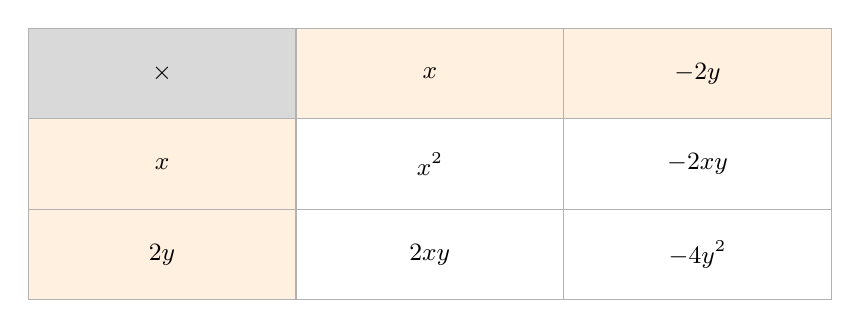
\begin{tikzpicture}[x=1cm,y=1cm,every node/.style={font=\small}]
\fill[gray!30] (0,0) rectangle (3.4,-1.15);
\draw[gray!60] (0,0) rectangle (3.4,-1.15);
\node at (1.7,-0.575) {$\displaystyle \times$};
\fill[orange!12] (3.4,0) rectangle (6.8,-1.15);
\draw[gray!60] (3.4,0) rectangle (6.8,-1.15);
\node at (5.1,-0.575) {$\displaystyle x$};
\fill[orange!12] (6.8,0) rectangle (10.2,-1.15);
\draw[gray!60] (6.8,0) rectangle (10.2,-1.15);
\node at (8.5,-0.575) {$\displaystyle -2y$};
\fill[orange!12] (0,-1.15) rectangle (3.4,-2.3);
\draw[gray!60] (0,-1.15) rectangle (3.4,-2.3);
\node at (1.7,-1.725) {$\displaystyle x$};
\fill[white] (3.4,-1.15) rectangle (6.8,-2.3);
\draw[gray!60] (3.4,-1.15) rectangle (6.8,-2.3);
\node at (5.1,-1.725) {$\displaystyle x^2$};
\fill[white] (6.8,-1.15) rectangle (10.2,-2.3);
\draw[gray!60] (6.8,-1.15) rectangle (10.2,-2.3);
\node at (8.5,-1.725) {$\displaystyle -2xy$};
\fill[orange!12] (0,-2.3) rectangle (3.4,-3.45);
\draw[gray!60] (0,-2.3) rectangle (3.4,-3.45);
\node at (1.7,-2.875) {$\displaystyle 2y$};
\fill[white] (3.4,-2.3) rectangle (6.8,-3.45);
\draw[gray!60] (3.4,-2.3) rectangle (6.8,-3.45);
\node at (5.1,-2.875) {$\displaystyle 2xy$};
\fill[white] (6.8,-2.3) rectangle (10.2,-3.45);
\draw[gray!60] (6.8,-2.3) rectangle (10.2,-3.45);
\node at (8.5,-2.875) {$\displaystyle -4y^2$};
\end{tikzpicture}
\end{center}
\small Take out $8$ first: $8(x^2-4y^2)$, then DOTS.\normalsize

\medskip\hrule

\section*{Factorising 28\quad\small\texttt{(a2-028)}}
\addcontentsline{toc}{section}{Factorising 28 (a2-028)}
\textit{Difficulty: Foundation \quad\textbar\quad Marks: 2}

\question{Factorise by grouping: \( ax - bx + ay - by \)}

\textbf{Worked solution.}

\textit{Step 1: Group the first two terms and the last two terms, factorising each pair separately.}
\[\begin{gathered}
x(a - b) + y(a - b)
\end{gathered}\]
Extract \( x \) from the first pair and \( y \) from the second pair.

\textit{Step 2: Factor out the newly formed common binomial bracket \( (a - b) \).}
\[\begin{gathered}
(a - b)(x + y)
\end{gathered}\]
Combine the factored groups to leave a product of two brackets.

\begin{answerbox}
\textbf{Final answer:}\quad \(\displaystyle (a - b)(x + y)\)
\end{answerbox}
\textbf{Area-model diagram.}

\begin{center}
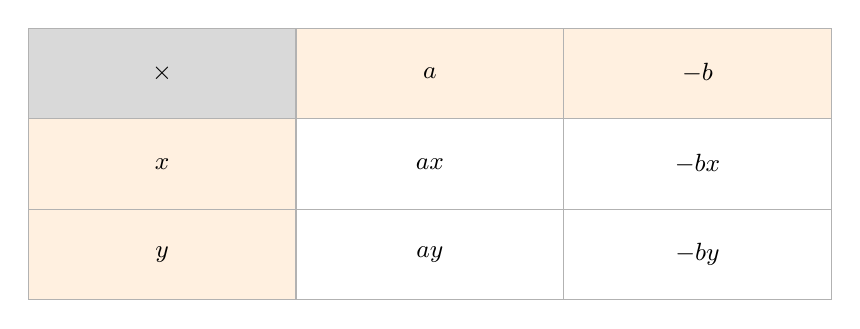
\begin{tikzpicture}[x=1cm,y=1cm,every node/.style={font=\small}]
\fill[gray!30] (0,0) rectangle (3.4,-1.15);
\draw[gray!60] (0,0) rectangle (3.4,-1.15);
\node at (1.7,-0.575) {$\displaystyle \times$};
\fill[orange!12] (3.4,0) rectangle (6.8,-1.15);
\draw[gray!60] (3.4,0) rectangle (6.8,-1.15);
\node at (5.1,-0.575) {$\displaystyle a$};
\fill[orange!12] (6.8,0) rectangle (10.2,-1.15);
\draw[gray!60] (6.8,0) rectangle (10.2,-1.15);
\node at (8.5,-0.575) {$\displaystyle -b$};
\fill[orange!12] (0,-1.15) rectangle (3.4,-2.3);
\draw[gray!60] (0,-1.15) rectangle (3.4,-2.3);
\node at (1.7,-1.725) {$\displaystyle x$};
\fill[white] (3.4,-1.15) rectangle (6.8,-2.3);
\draw[gray!60] (3.4,-1.15) rectangle (6.8,-2.3);
\node at (5.1,-1.725) {$\displaystyle ax$};
\fill[white] (6.8,-1.15) rectangle (10.2,-2.3);
\draw[gray!60] (6.8,-1.15) rectangle (10.2,-2.3);
\node at (8.5,-1.725) {$\displaystyle -bx$};
\fill[orange!12] (0,-2.3) rectangle (3.4,-3.45);
\draw[gray!60] (0,-2.3) rectangle (3.4,-3.45);
\node at (1.7,-2.875) {$\displaystyle y$};
\fill[white] (3.4,-2.3) rectangle (6.8,-3.45);
\draw[gray!60] (3.4,-2.3) rectangle (6.8,-3.45);
\node at (5.1,-2.875) {$\displaystyle ay$};
\fill[white] (6.8,-2.3) rectangle (10.2,-3.45);
\draw[gray!60] (6.8,-2.3) rectangle (10.2,-3.45);
\node at (8.5,-2.875) {$\displaystyle -by$};
\end{tikzpicture}
\end{center}
\small Grouping: $x(a-b)+y(a-b)=(x+y)(a-b)$.\normalsize

\medskip\hrule

\section*{Factorising 29\quad\small\texttt{(a2-029)}}
\addcontentsline{toc}{section}{Factorising 29 (a2-029)}
\textit{Difficulty: Foundation \quad\textbar\quad Marks: 3}

\question{Express as the product of factors: \( 2u(v-w) + 5(w-v) \)}

\textbf{Worked solution.}

\textit{Step 1: Notice the brackets \( (v-w) \) and \( (w-v) \) are opposites. Factor out -1 from the second term to make them identical.}
\[\begin{gathered}
2u(v-w) - 5(v-w)
\end{gathered}\]
Reverse the sign of the second term to reveal a common bracket.

\textit{Step 2: Factor out the common bracket \( (v-w) \).}
\[\begin{gathered}
(v-w)(2u - 5)
\end{gathered}\]
Extract the shared binomial factor.

\begin{answerbox}
\textbf{Final answer:}\quad \(\displaystyle (v-w)(2u - 5)\)
\end{answerbox}
\textbf{Area-model diagram.}

\begin{center}
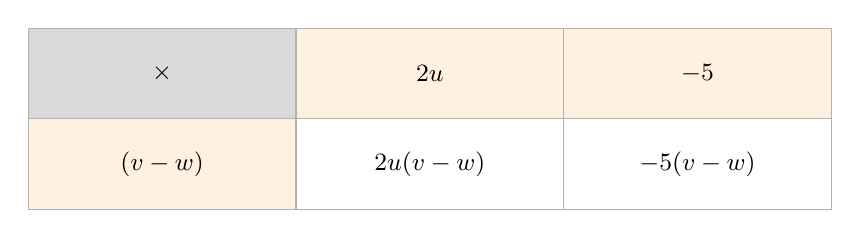
\begin{tikzpicture}[x=1cm,y=1cm,every node/.style={font=\small}]
\fill[gray!30] (0,0) rectangle (3.4,-1.15);
\draw[gray!60] (0,0) rectangle (3.4,-1.15);
\node at (1.7,-0.575) {$\displaystyle \times$};
\fill[orange!12] (3.4,0) rectangle (6.8,-1.15);
\draw[gray!60] (3.4,0) rectangle (6.8,-1.15);
\node at (5.1,-0.575) {$\displaystyle 2u$};
\fill[orange!12] (6.8,0) rectangle (10.2,-1.15);
\draw[gray!60] (6.8,0) rectangle (10.2,-1.15);
\node at (8.5,-0.575) {$\displaystyle -5$};
\fill[orange!12] (0,-1.15) rectangle (3.4,-2.3);
\draw[gray!60] (0,-1.15) rectangle (3.4,-2.3);
\node at (1.7,-1.725) {$\displaystyle (v-w)$};
\fill[white] (3.4,-1.15) rectangle (6.8,-2.3);
\draw[gray!60] (3.4,-1.15) rectangle (6.8,-2.3);
\node at (5.1,-1.725) {$\displaystyle 2u(v-w)$};
\fill[white] (6.8,-1.15) rectangle (10.2,-2.3);
\draw[gray!60] (6.8,-1.15) rectangle (10.2,-2.3);
\node at (8.5,-1.725) {$\displaystyle -5(v-w)$};
\end{tikzpicture}
\end{center}
\small Rewrite $5(w-v)=-5(v-w)$ to expose the common bracket $(v-w)$.\normalsize

\medskip\hrule

\section*{Factorising 30\quad\small\texttt{(a2-030)}}
\addcontentsline{toc}{section}{Factorising 30 (a2-030)}
\textit{Difficulty: Foundation \quad\textbar\quad Marks: 2}

\question{Simplify the expression, leaving your answer in factorised form: \( (p+q)^2 - 3(p+q) \)}

\textbf{Worked solution.}

\textit{Step 1: Identify that \( (p+q) \) is a common factor in both terms.}
\[\begin{gathered}
(p+q)[(p+q) - 3]
\end{gathered}\]
Pull the shared bracket out to the front.

\textit{Step 2: Remove the inner square brackets to give the final simplified expression.}
\[\begin{gathered}
(p+q)(p+q-3)
\end{gathered}\]
Neaten up the expression.

\begin{answerbox}
\textbf{Final answer:}\quad \(\displaystyle (p+q)(p+q-3)\)
\end{answerbox}
\textbf{Area-model diagram.}

\begin{center}
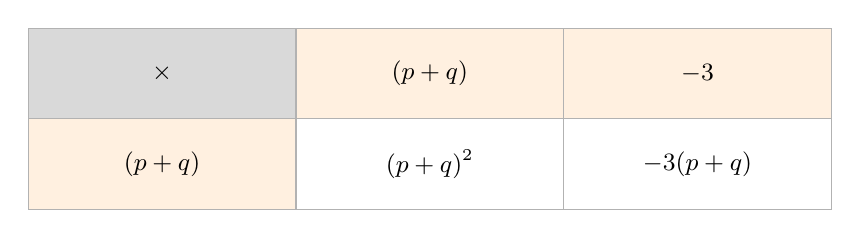
\begin{tikzpicture}[x=1cm,y=1cm,every node/.style={font=\small}]
\fill[gray!30] (0,0) rectangle (3.4,-1.15);
\draw[gray!60] (0,0) rectangle (3.4,-1.15);
\node at (1.7,-0.575) {$\displaystyle \times$};
\fill[orange!12] (3.4,0) rectangle (6.8,-1.15);
\draw[gray!60] (3.4,0) rectangle (6.8,-1.15);
\node at (5.1,-0.575) {$\displaystyle (p+q)$};
\fill[orange!12] (6.8,0) rectangle (10.2,-1.15);
\draw[gray!60] (6.8,0) rectangle (10.2,-1.15);
\node at (8.5,-0.575) {$\displaystyle -3$};
\fill[orange!12] (0,-1.15) rectangle (3.4,-2.3);
\draw[gray!60] (0,-1.15) rectangle (3.4,-2.3);
\node at (1.7,-1.725) {$\displaystyle (p+q)$};
\fill[white] (3.4,-1.15) rectangle (6.8,-2.3);
\draw[gray!60] (3.4,-1.15) rectangle (6.8,-2.3);
\node at (5.1,-1.725) {$\displaystyle (p+q)^2$};
\fill[white] (6.8,-1.15) rectangle (10.2,-2.3);
\draw[gray!60] (6.8,-1.15) rectangle (10.2,-2.3);
\node at (8.5,-1.725) {$\displaystyle -3(p+q)$};
\end{tikzpicture}
\end{center}
\small Common bracket $(p+q)$.\normalsize

\medskip\hrule

\section*{Factorising 31\quad\small\texttt{(a2-031)}}
\addcontentsline{toc}{section}{Factorising 31 (a2-031)}
\textit{Difficulty: Foundation \quad\textbar\quad Marks: 1}

\question{Factorise: \( 18p - 27q \)}

\textbf{Worked solution.}

\textit{Find the highest common factor (HCF) of 18 and 27, which is 9.}
\[\begin{gathered}
9(2p - 3q)
\end{gathered}\]
Divide both terms by 9 to find the expression inside the bracket.

\begin{answerbox}
\textbf{Final answer:}\quad \(\displaystyle 9(2p - 3q)\)
\end{answerbox}
\textbf{Area-model diagram.}

\begin{center}
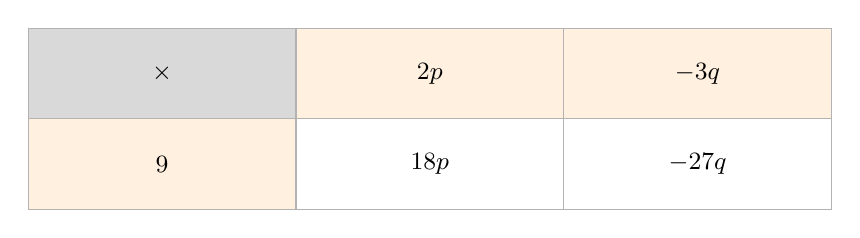
\begin{tikzpicture}[x=1cm,y=1cm,every node/.style={font=\small}]
\fill[gray!30] (0,0) rectangle (3.4,-1.15);
\draw[gray!60] (0,0) rectangle (3.4,-1.15);
\node at (1.7,-0.575) {$\displaystyle \times$};
\fill[orange!12] (3.4,0) rectangle (6.8,-1.15);
\draw[gray!60] (3.4,0) rectangle (6.8,-1.15);
\node at (5.1,-0.575) {$\displaystyle 2p$};
\fill[orange!12] (6.8,0) rectangle (10.2,-1.15);
\draw[gray!60] (6.8,0) rectangle (10.2,-1.15);
\node at (8.5,-0.575) {$\displaystyle -3q$};
\fill[orange!12] (0,-1.15) rectangle (3.4,-2.3);
\draw[gray!60] (0,-1.15) rectangle (3.4,-2.3);
\node at (1.7,-1.725) {$\displaystyle 9$};
\fill[white] (3.4,-1.15) rectangle (6.8,-2.3);
\draw[gray!60] (3.4,-1.15) rectangle (6.8,-2.3);
\node at (5.1,-1.725) {$\displaystyle 18p$};
\fill[white] (6.8,-1.15) rectangle (10.2,-2.3);
\draw[gray!60] (6.8,-1.15) rectangle (10.2,-2.3);
\node at (8.5,-1.725) {$\displaystyle -27q$};
\end{tikzpicture}
\end{center}
\small HCF $9$.\normalsize

\medskip\hrule

\section*{Factorising 32\quad\small\texttt{(a2-032)}}
\addcontentsline{toc}{section}{Factorising 32 (a2-032)}
\textit{Difficulty: Foundation \quad\textbar\quad Marks: 2}

\question{Write the expression as a product of factors: \( 4c^2 - d^2 \)}

\textbf{Worked solution.}

\textit{Recognise this as a difference of two squares, rewriting the terms as \( (2c)^2 \) and \( d^2 \).}
\[\begin{gathered}
(2c)^2 - d^2
\end{gathered}\]
Identify the squared components to apply the rule \( A^2 - B^2 = (A-B)(A+B) \).

\begin{answerbox}
\textbf{Final answer:}\quad \(\displaystyle (2c - d)(2c + d)\)
\end{answerbox}
\textbf{Area-model diagram.}

\begin{center}
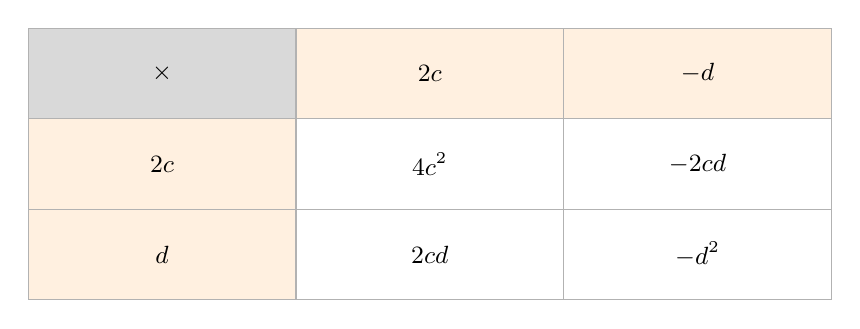
\begin{tikzpicture}[x=1cm,y=1cm,every node/.style={font=\small}]
\fill[gray!30] (0,0) rectangle (3.4,-1.15);
\draw[gray!60] (0,0) rectangle (3.4,-1.15);
\node at (1.7,-0.575) {$\displaystyle \times$};
\fill[orange!12] (3.4,0) rectangle (6.8,-1.15);
\draw[gray!60] (3.4,0) rectangle (6.8,-1.15);
\node at (5.1,-0.575) {$\displaystyle 2c$};
\fill[orange!12] (6.8,0) rectangle (10.2,-1.15);
\draw[gray!60] (6.8,0) rectangle (10.2,-1.15);
\node at (8.5,-0.575) {$\displaystyle -d$};
\fill[orange!12] (0,-1.15) rectangle (3.4,-2.3);
\draw[gray!60] (0,-1.15) rectangle (3.4,-2.3);
\node at (1.7,-1.725) {$\displaystyle 2c$};
\fill[white] (3.4,-1.15) rectangle (6.8,-2.3);
\draw[gray!60] (3.4,-1.15) rectangle (6.8,-2.3);
\node at (5.1,-1.725) {$\displaystyle 4c^2$};
\fill[white] (6.8,-1.15) rectangle (10.2,-2.3);
\draw[gray!60] (6.8,-1.15) rectangle (10.2,-2.3);
\node at (8.5,-1.725) {$\displaystyle -2cd$};
\fill[orange!12] (0,-2.3) rectangle (3.4,-3.45);
\draw[gray!60] (0,-2.3) rectangle (3.4,-3.45);
\node at (1.7,-2.875) {$\displaystyle d$};
\fill[white] (3.4,-2.3) rectangle (6.8,-3.45);
\draw[gray!60] (3.4,-2.3) rectangle (6.8,-3.45);
\node at (5.1,-2.875) {$\displaystyle 2cd$};
\fill[white] (6.8,-2.3) rectangle (10.2,-3.45);
\draw[gray!60] (6.8,-2.3) rectangle (10.2,-3.45);
\node at (8.5,-2.875) {$\displaystyle -d^2$};
\end{tikzpicture}
\end{center}
\small DOTS: $4c^2=(2c)^2$.\normalsize

\medskip\hrule

\section*{Factorising 33\quad\small\texttt{(a2-033)}}
\addcontentsline{toc}{section}{Factorising 33 (a2-033)}
\textit{Difficulty: Foundation \quad\textbar\quad Marks: 2}

\question{Factorise fully: \( 5x^2y + 15xy^2 - 10xy \)}

\textbf{Worked solution.}

\textit{Step 1: Identify the highest common numerical factor (which is 5) and the shared variables (which are \( x \) and \( y \)).}
\[\begin{gathered}
5xy
\end{gathered}\]
Find the greatest term that divides exactly into all three parts of the expression.

\textit{Step 2: Factor out \( 5xy \) from the original expression.}
\[\begin{gathered}
5xy(x + 3y - 2)
\end{gathered}\]
Divide each original term by the common factor to populate the bracket.

\begin{answerbox}
\textbf{Final answer:}\quad \(\displaystyle 5xy(x + 3y - 2)\)
\end{answerbox}
\textbf{Area-model diagram.}

\begin{center}
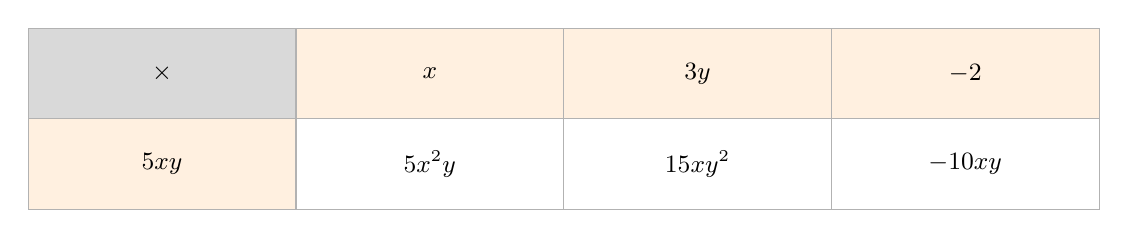
\begin{tikzpicture}[x=1cm,y=1cm,every node/.style={font=\small}]
\fill[gray!30] (0,0) rectangle (3.4,-1.15);
\draw[gray!60] (0,0) rectangle (3.4,-1.15);
\node at (1.7,-0.575) {$\displaystyle \times$};
\fill[orange!12] (3.4,0) rectangle (6.8,-1.15);
\draw[gray!60] (3.4,0) rectangle (6.8,-1.15);
\node at (5.1,-0.575) {$\displaystyle x$};
\fill[orange!12] (6.8,0) rectangle (10.2,-1.15);
\draw[gray!60] (6.8,0) rectangle (10.2,-1.15);
\node at (8.5,-0.575) {$\displaystyle 3y$};
\fill[orange!12] (10.2,0) rectangle (13.6,-1.15);
\draw[gray!60] (10.2,0) rectangle (13.6,-1.15);
\node at (11.9,-0.575) {$\displaystyle -2$};
\fill[orange!12] (0,-1.15) rectangle (3.4,-2.3);
\draw[gray!60] (0,-1.15) rectangle (3.4,-2.3);
\node at (1.7,-1.725) {$\displaystyle 5xy$};
\fill[white] (3.4,-1.15) rectangle (6.8,-2.3);
\draw[gray!60] (3.4,-1.15) rectangle (6.8,-2.3);
\node at (5.1,-1.725) {$\displaystyle 5x^2y$};
\fill[white] (6.8,-1.15) rectangle (10.2,-2.3);
\draw[gray!60] (6.8,-1.15) rectangle (10.2,-2.3);
\node at (8.5,-1.725) {$\displaystyle 15xy^2$};
\fill[white] (10.2,-1.15) rectangle (13.6,-2.3);
\draw[gray!60] (10.2,-1.15) rectangle (13.6,-2.3);
\node at (11.9,-1.725) {$\displaystyle -10xy$};
\end{tikzpicture}
\end{center}
\small HCF $5xy$; three-term bracket.\normalsize

\medskip\hrule

\section*{Factorising 34\quad\small\texttt{(a2-034)}}
\addcontentsline{toc}{section}{Factorising 34 (a2-034)}
\textit{Difficulty: Foundation \quad\textbar\quad Marks: 2}

\question{Express as the product of factors: \( m(n-2) + 4(n-2) \)}

\textbf{Worked solution.}

\textit{Identify that the binomial \( (n-2) \) is a common factor in both terms.}
\[\begin{gathered}
(n-2)(m + 4)
\end{gathered}\]
Extract the shared bracket to the front and group the remaining outer terms into a second bracket.

\begin{answerbox}
\textbf{Final answer:}\quad \(\displaystyle (n-2)(m + 4)\)
\end{answerbox}
\textbf{Area-model diagram.}

\begin{center}
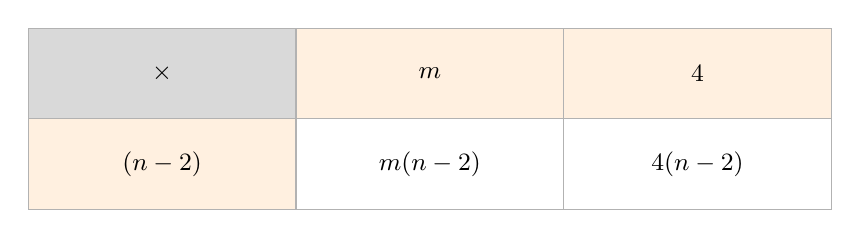
\begin{tikzpicture}[x=1cm,y=1cm,every node/.style={font=\small}]
\fill[gray!30] (0,0) rectangle (3.4,-1.15);
\draw[gray!60] (0,0) rectangle (3.4,-1.15);
\node at (1.7,-0.575) {$\displaystyle \times$};
\fill[orange!12] (3.4,0) rectangle (6.8,-1.15);
\draw[gray!60] (3.4,0) rectangle (6.8,-1.15);
\node at (5.1,-0.575) {$\displaystyle m$};
\fill[orange!12] (6.8,0) rectangle (10.2,-1.15);
\draw[gray!60] (6.8,0) rectangle (10.2,-1.15);
\node at (8.5,-0.575) {$\displaystyle 4$};
\fill[orange!12] (0,-1.15) rectangle (3.4,-2.3);
\draw[gray!60] (0,-1.15) rectangle (3.4,-2.3);
\node at (1.7,-1.725) {$\displaystyle (n-2)$};
\fill[white] (3.4,-1.15) rectangle (6.8,-2.3);
\draw[gray!60] (3.4,-1.15) rectangle (6.8,-2.3);
\node at (5.1,-1.725) {$\displaystyle m(n-2)$};
\fill[white] (6.8,-1.15) rectangle (10.2,-2.3);
\draw[gray!60] (6.8,-1.15) rectangle (10.2,-2.3);
\node at (8.5,-1.725) {$\displaystyle 4(n-2)$};
\end{tikzpicture}
\end{center}
\small Common bracket $(n-2)$.\normalsize

\medskip\hrule

\section*{Factorising 35\quad\small\texttt{(a2-035)}}
\addcontentsline{toc}{section}{Factorising 35 (a2-035)}
\textit{Difficulty: Foundation \quad\textbar\quad Marks: 3}

\question{Factorise completely: \( 12a^2 - 75b^2 \)}

\textbf{Worked solution.}

\textit{Step 1: Extract the highest common numerical factor of 3 from both terms first.}
\[\begin{gathered}
3(4a^2 - 25b^2)
\end{gathered}\]
Always check for a common factor before applying difference of two squares.

\textit{Step 2: Recognise that the expression inside the bracket is a difference of two squares and factorise it.}
\[\begin{gathered}
3(2a - 5b)(2a + 5b)
\end{gathered}\]
Apply the pattern \( A^2 - B^2 = (A-B)(A+B) \) to the inner quadratic.

\begin{answerbox}
\textbf{Final answer:}\quad \(\displaystyle 3(2a - 5b)(2a + 5b)\)
\end{answerbox}
\textbf{Area-model diagram.}

\begin{center}
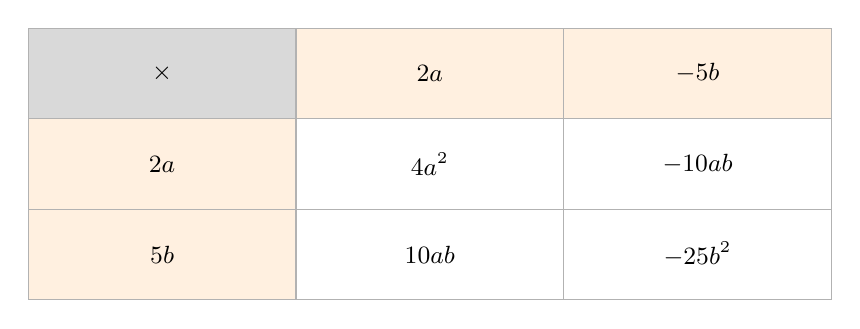
\begin{tikzpicture}[x=1cm,y=1cm,every node/.style={font=\small}]
\fill[gray!30] (0,0) rectangle (3.4,-1.15);
\draw[gray!60] (0,0) rectangle (3.4,-1.15);
\node at (1.7,-0.575) {$\displaystyle \times$};
\fill[orange!12] (3.4,0) rectangle (6.8,-1.15);
\draw[gray!60] (3.4,0) rectangle (6.8,-1.15);
\node at (5.1,-0.575) {$\displaystyle 2a$};
\fill[orange!12] (6.8,0) rectangle (10.2,-1.15);
\draw[gray!60] (6.8,0) rectangle (10.2,-1.15);
\node at (8.5,-0.575) {$\displaystyle -5b$};
\fill[orange!12] (0,-1.15) rectangle (3.4,-2.3);
\draw[gray!60] (0,-1.15) rectangle (3.4,-2.3);
\node at (1.7,-1.725) {$\displaystyle 2a$};
\fill[white] (3.4,-1.15) rectangle (6.8,-2.3);
\draw[gray!60] (3.4,-1.15) rectangle (6.8,-2.3);
\node at (5.1,-1.725) {$\displaystyle 4a^2$};
\fill[white] (6.8,-1.15) rectangle (10.2,-2.3);
\draw[gray!60] (6.8,-1.15) rectangle (10.2,-2.3);
\node at (8.5,-1.725) {$\displaystyle -10ab$};
\fill[orange!12] (0,-2.3) rectangle (3.4,-3.45);
\draw[gray!60] (0,-2.3) rectangle (3.4,-3.45);
\node at (1.7,-2.875) {$\displaystyle 5b$};
\fill[white] (3.4,-2.3) rectangle (6.8,-3.45);
\draw[gray!60] (3.4,-2.3) rectangle (6.8,-3.45);
\node at (5.1,-2.875) {$\displaystyle 10ab$};
\fill[white] (6.8,-2.3) rectangle (10.2,-3.45);
\draw[gray!60] (6.8,-2.3) rectangle (10.2,-3.45);
\node at (8.5,-2.875) {$\displaystyle -25b^2$};
\end{tikzpicture}
\end{center}
\small Take out $3$ first: $3(4a^2-25b^2)$, then DOTS.\normalsize

\medskip\hrule

\section*{Factorising 36\quad\small\texttt{(a2-036)}}
\addcontentsline{toc}{section}{Factorising 36 (a2-036)}
\textit{Difficulty: Foundation \quad\textbar\quad Marks: 2}

\question{Factorise by grouping: \( pr + ps + qr + qs \)}

\textbf{Worked solution.}

\textit{Step 1: Group the first two terms and the last two terms, then factorise each pair.}
\[\begin{gathered}
p(r + s) + q(r + s)
\end{gathered}\]
Extract \( p \) from the first pair and \( q \) from the second pair.

\textit{Step 2: Factor out the newly formed common binomial bracket \( (r + s) \).}
\[\begin{gathered}
(r + s)(p + q)
\end{gathered}\]
Combine the factored groups together.

\begin{answerbox}
\textbf{Final answer:}\quad \(\displaystyle (r + s)(p + q)\)
\end{answerbox}
\textbf{Area-model diagram.}

\begin{center}
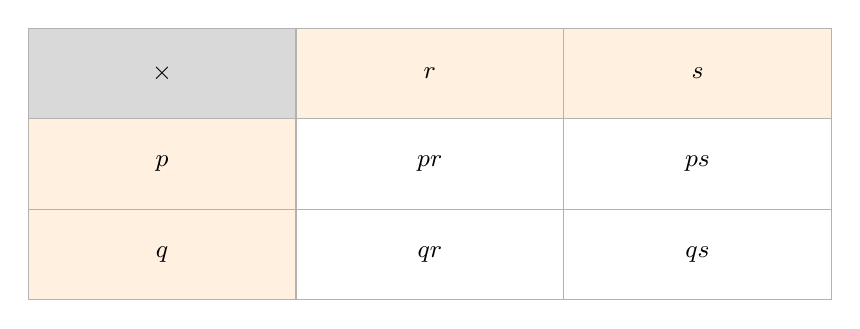
\begin{tikzpicture}[x=1cm,y=1cm,every node/.style={font=\small}]
\fill[gray!30] (0,0) rectangle (3.4,-1.15);
\draw[gray!60] (0,0) rectangle (3.4,-1.15);
\node at (1.7,-0.575) {$\displaystyle \times$};
\fill[orange!12] (3.4,0) rectangle (6.8,-1.15);
\draw[gray!60] (3.4,0) rectangle (6.8,-1.15);
\node at (5.1,-0.575) {$\displaystyle r$};
\fill[orange!12] (6.8,0) rectangle (10.2,-1.15);
\draw[gray!60] (6.8,0) rectangle (10.2,-1.15);
\node at (8.5,-0.575) {$\displaystyle s$};
\fill[orange!12] (0,-1.15) rectangle (3.4,-2.3);
\draw[gray!60] (0,-1.15) rectangle (3.4,-2.3);
\node at (1.7,-1.725) {$\displaystyle p$};
\fill[white] (3.4,-1.15) rectangle (6.8,-2.3);
\draw[gray!60] (3.4,-1.15) rectangle (6.8,-2.3);
\node at (5.1,-1.725) {$\displaystyle pr$};
\fill[white] (6.8,-1.15) rectangle (10.2,-2.3);
\draw[gray!60] (6.8,-1.15) rectangle (10.2,-2.3);
\node at (8.5,-1.725) {$\displaystyle ps$};
\fill[orange!12] (0,-2.3) rectangle (3.4,-3.45);
\draw[gray!60] (0,-2.3) rectangle (3.4,-3.45);
\node at (1.7,-2.875) {$\displaystyle q$};
\fill[white] (3.4,-2.3) rectangle (6.8,-3.45);
\draw[gray!60] (3.4,-2.3) rectangle (6.8,-3.45);
\node at (5.1,-2.875) {$\displaystyle qr$};
\fill[white] (6.8,-2.3) rectangle (10.2,-3.45);
\draw[gray!60] (6.8,-2.3) rectangle (10.2,-3.45);
\node at (8.5,-2.875) {$\displaystyle qs$};
\end{tikzpicture}
\end{center}
\small Grouping: $p(r+s)+q(r+s)=(p+q)(r+s)$.\normalsize

\medskip\hrule

\section*{Factorising 37\quad\small\texttt{(a2-037)}}
\addcontentsline{toc}{section}{Factorising 37 (a2-037)}
\textit{Difficulty: Foundation \quad\textbar\quad Marks: 3}

\question{Simplify the expression, leaving your answer in factorised form: \( (2x-y)^2 - x(2x-y) \)}

\textbf{Worked solution.}

\textit{Step 1: Identify that \( (2x-y) \) is a common factor in both terms and extract it.}
\[\begin{gathered}
(2x-y)[(2x-y) - x]
\end{gathered}\]
Pull the shared binomial bracket out to the front.

\textit{Step 2: Simplify the expression inside the square brackets by collecting like terms: \( 2x - y - x = x - y \).}
\[\begin{gathered}
(2x-y)(x-y)
\end{gathered}\]
Neaten up the second bracket to find the final factorised form.

\begin{answerbox}
\textbf{Final answer:}\quad \(\displaystyle (2x-y)(x-y)\)
\end{answerbox}
\textbf{Area-model diagram.}

\begin{center}
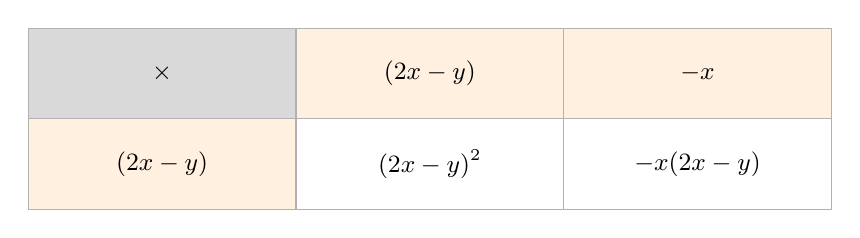
\begin{tikzpicture}[x=1cm,y=1cm,every node/.style={font=\small}]
\fill[gray!30] (0,0) rectangle (3.4,-1.15);
\draw[gray!60] (0,0) rectangle (3.4,-1.15);
\node at (1.7,-0.575) {$\displaystyle \times$};
\fill[orange!12] (3.4,0) rectangle (6.8,-1.15);
\draw[gray!60] (3.4,0) rectangle (6.8,-1.15);
\node at (5.1,-0.575) {$\displaystyle (2x-y)$};
\fill[orange!12] (6.8,0) rectangle (10.2,-1.15);
\draw[gray!60] (6.8,0) rectangle (10.2,-1.15);
\node at (8.5,-0.575) {$\displaystyle -x$};
\fill[orange!12] (0,-1.15) rectangle (3.4,-2.3);
\draw[gray!60] (0,-1.15) rectangle (3.4,-2.3);
\node at (1.7,-1.725) {$\displaystyle (2x-y)$};
\fill[white] (3.4,-1.15) rectangle (6.8,-2.3);
\draw[gray!60] (3.4,-1.15) rectangle (6.8,-2.3);
\node at (5.1,-1.725) {$\displaystyle (2x-y)^2$};
\fill[white] (6.8,-1.15) rectangle (10.2,-2.3);
\draw[gray!60] (6.8,-1.15) rectangle (10.2,-2.3);
\node at (8.5,-1.725) {$\displaystyle -x(2x-y)$};
\end{tikzpicture}
\end{center}
\small Common bracket $(2x-y)$; then $(2x-y)-x=(x-y)$.\normalsize

\medskip\hrule

\section*{Factorising 38\quad\small\texttt{(a2-038)}}
\addcontentsline{toc}{section}{Factorising 38 (a2-038)}
\textit{Difficulty: Foundation \quad\textbar\quad Marks: 1}

\question{Factorise completely: \( 24u + 36v \)}

\textbf{Worked solution.}

\textit{Identify the highest common factor (HCF) of the numbers 24 and 36, which is 12.}
\[\begin{gathered}
12(2u + 3v)
\end{gathered}\]
Divide both terms by 12 and place the remaining expression inside the bracket.

\begin{answerbox}
\textbf{Final answer:}\quad \(\displaystyle 12(2u + 3v)\)
\end{answerbox}
\textbf{Area-model diagram.}

\begin{center}
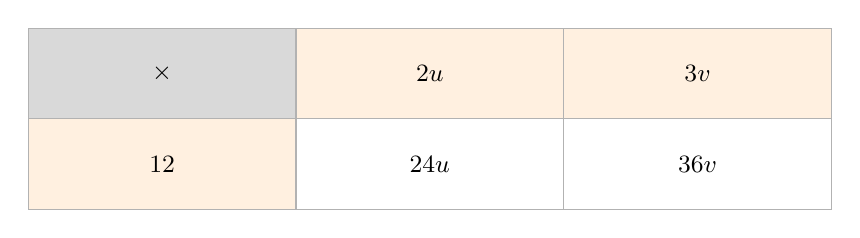
\begin{tikzpicture}[x=1cm,y=1cm,every node/.style={font=\small}]
\fill[gray!30] (0,0) rectangle (3.4,-1.15);
\draw[gray!60] (0,0) rectangle (3.4,-1.15);
\node at (1.7,-0.575) {$\displaystyle \times$};
\fill[orange!12] (3.4,0) rectangle (6.8,-1.15);
\draw[gray!60] (3.4,0) rectangle (6.8,-1.15);
\node at (5.1,-0.575) {$\displaystyle 2u$};
\fill[orange!12] (6.8,0) rectangle (10.2,-1.15);
\draw[gray!60] (6.8,0) rectangle (10.2,-1.15);
\node at (8.5,-0.575) {$\displaystyle 3v$};
\fill[orange!12] (0,-1.15) rectangle (3.4,-2.3);
\draw[gray!60] (0,-1.15) rectangle (3.4,-2.3);
\node at (1.7,-1.725) {$\displaystyle 12$};
\fill[white] (3.4,-1.15) rectangle (6.8,-2.3);
\draw[gray!60] (3.4,-1.15) rectangle (6.8,-2.3);
\node at (5.1,-1.725) {$\displaystyle 24u$};
\fill[white] (6.8,-1.15) rectangle (10.2,-2.3);
\draw[gray!60] (6.8,-1.15) rectangle (10.2,-2.3);
\node at (8.5,-1.725) {$\displaystyle 36v$};
\end{tikzpicture}
\end{center}
\small HCF $12$.\normalsize

\medskip\hrule

\section*{Factorising 39\quad\small\texttt{(a2-039)}}
\addcontentsline{toc}{section}{Factorising 39 (a2-039)}
\textit{Difficulty: Foundation \quad\textbar\quad Marks: 2}

\question{Write the expression as a product of factors: \( 49x^2 - y^2 \)}

\textbf{Worked solution.}

\textit{Recognise that this is a difference of two squares, rewriting the first term as \( (7x)^2 \).}
\[\begin{gathered}
(7x)^2 - y^2
\end{gathered}\]
Identify the squared components to apply the rule \( A^2 - B^2 = (A-B)(A+B) \).

\begin{answerbox}
\textbf{Final answer:}\quad \(\displaystyle (7x - y)(7x + y)\)
\end{answerbox}
\textbf{Area-model diagram.}

\begin{center}
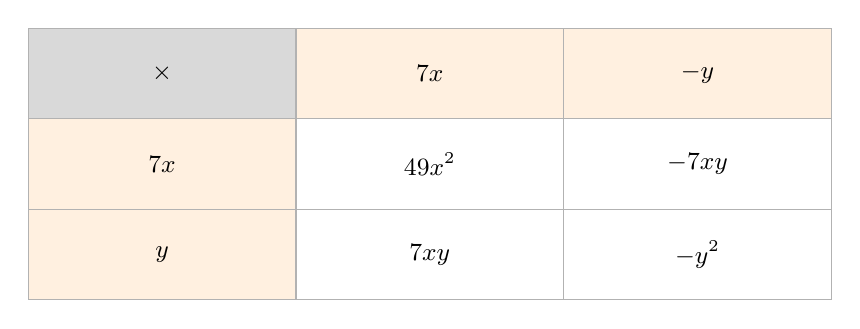
\begin{tikzpicture}[x=1cm,y=1cm,every node/.style={font=\small}]
\fill[gray!30] (0,0) rectangle (3.4,-1.15);
\draw[gray!60] (0,0) rectangle (3.4,-1.15);
\node at (1.7,-0.575) {$\displaystyle \times$};
\fill[orange!12] (3.4,0) rectangle (6.8,-1.15);
\draw[gray!60] (3.4,0) rectangle (6.8,-1.15);
\node at (5.1,-0.575) {$\displaystyle 7x$};
\fill[orange!12] (6.8,0) rectangle (10.2,-1.15);
\draw[gray!60] (6.8,0) rectangle (10.2,-1.15);
\node at (8.5,-0.575) {$\displaystyle -y$};
\fill[orange!12] (0,-1.15) rectangle (3.4,-2.3);
\draw[gray!60] (0,-1.15) rectangle (3.4,-2.3);
\node at (1.7,-1.725) {$\displaystyle 7x$};
\fill[white] (3.4,-1.15) rectangle (6.8,-2.3);
\draw[gray!60] (3.4,-1.15) rectangle (6.8,-2.3);
\node at (5.1,-1.725) {$\displaystyle 49x^2$};
\fill[white] (6.8,-1.15) rectangle (10.2,-2.3);
\draw[gray!60] (6.8,-1.15) rectangle (10.2,-2.3);
\node at (8.5,-1.725) {$\displaystyle -7xy$};
\fill[orange!12] (0,-2.3) rectangle (3.4,-3.45);
\draw[gray!60] (0,-2.3) rectangle (3.4,-3.45);
\node at (1.7,-2.875) {$\displaystyle y$};
\fill[white] (3.4,-2.3) rectangle (6.8,-3.45);
\draw[gray!60] (3.4,-2.3) rectangle (6.8,-3.45);
\node at (5.1,-2.875) {$\displaystyle 7xy$};
\fill[white] (6.8,-2.3) rectangle (10.2,-3.45);
\draw[gray!60] (6.8,-2.3) rectangle (10.2,-3.45);
\node at (8.5,-2.875) {$\displaystyle -y^2$};
\end{tikzpicture}
\end{center}
\small DOTS: $49x^2=(7x)^2$.\normalsize

\medskip\hrule

\section*{Factorising 40\quad\small\texttt{(a2-040)}}
\addcontentsline{toc}{section}{Factorising 40 (a2-040)}
\textit{Difficulty: Foundation \quad\textbar\quad Marks: 2}

\question{Factorise fully: \( 16a^3b^2 - 24a^2b^3 \)}

\textbf{Worked solution.}

\textit{Step 1: Identify the highest common numerical factor (which is 8) and the highest common powers of the variables (which are \( a^2 \) and \( b^2 \)).}
\[\begin{gathered}
8a^2b^2
\end{gathered}\]
Find the greatest algebraic term that divides exactly into both parts of the expression.

\textit{Step 2: Factor out \( 8a^2b^2 \) from the original expression.}
\[\begin{gathered}
8a^2b^2(2a - 3b)
\end{gathered}\]
Divide each original term by the common factor to populate the bracket.

\begin{answerbox}
\textbf{Final answer:}\quad \(\displaystyle 8a^2b^2(2a - 3b)\)
\end{answerbox}
\textbf{Area-model diagram.}

\begin{center}
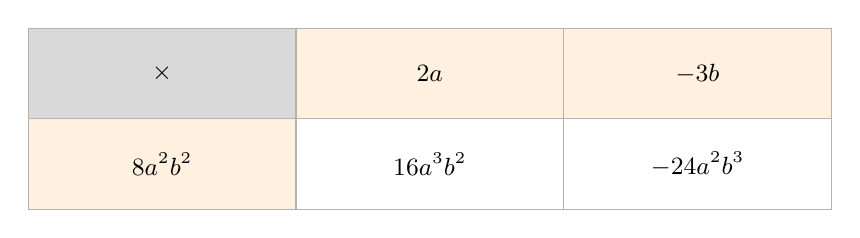
\begin{tikzpicture}[x=1cm,y=1cm,every node/.style={font=\small}]
\fill[gray!30] (0,0) rectangle (3.4,-1.15);
\draw[gray!60] (0,0) rectangle (3.4,-1.15);
\node at (1.7,-0.575) {$\displaystyle \times$};
\fill[orange!12] (3.4,0) rectangle (6.8,-1.15);
\draw[gray!60] (3.4,0) rectangle (6.8,-1.15);
\node at (5.1,-0.575) {$\displaystyle 2a$};
\fill[orange!12] (6.8,0) rectangle (10.2,-1.15);
\draw[gray!60] (6.8,0) rectangle (10.2,-1.15);
\node at (8.5,-0.575) {$\displaystyle -3b$};
\fill[orange!12] (0,-1.15) rectangle (3.4,-2.3);
\draw[gray!60] (0,-1.15) rectangle (3.4,-2.3);
\node at (1.7,-1.725) {$\displaystyle 8a^2b^2$};
\fill[white] (3.4,-1.15) rectangle (6.8,-2.3);
\draw[gray!60] (3.4,-1.15) rectangle (6.8,-2.3);
\node at (5.1,-1.725) {$\displaystyle 16a^3b^2$};
\fill[white] (6.8,-1.15) rectangle (10.2,-2.3);
\draw[gray!60] (6.8,-1.15) rectangle (10.2,-2.3);
\node at (8.5,-1.725) {$\displaystyle -24a^2b^3$};
\end{tikzpicture}
\end{center}
\small HCF $8a^2b^2$.\normalsize

\medskip\hrule

\section*{Factorising 41\quad\small\texttt{(a2-041)}}
\addcontentsline{toc}{section}{Factorising 41 (a2-041)}
\textit{Difficulty: Foundation \quad\textbar\quad Marks: 2}

\question{Express as the product of factors: \( x(y+5) - 2(y+5) \)}

\textbf{Worked solution.}

\textit{Identify that the binomial \( (y+5) \) is a common factor in both terms.}
\[\begin{gathered}
(y+5)(x - 2)
\end{gathered}\]
Extract the shared bracket to the front and group the remaining outer multipliers into a second bracket.

\begin{answerbox}
\textbf{Final answer:}\quad \(\displaystyle (y+5)(x - 2)\)
\end{answerbox}
\textbf{Area-model diagram.}

\begin{center}
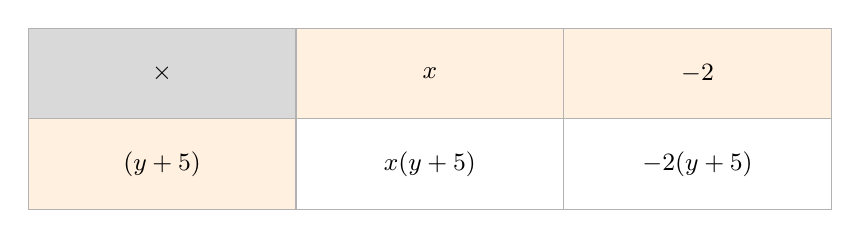
\begin{tikzpicture}[x=1cm,y=1cm,every node/.style={font=\small}]
\fill[gray!30] (0,0) rectangle (3.4,-1.15);
\draw[gray!60] (0,0) rectangle (3.4,-1.15);
\node at (1.7,-0.575) {$\displaystyle \times$};
\fill[orange!12] (3.4,0) rectangle (6.8,-1.15);
\draw[gray!60] (3.4,0) rectangle (6.8,-1.15);
\node at (5.1,-0.575) {$\displaystyle x$};
\fill[orange!12] (6.8,0) rectangle (10.2,-1.15);
\draw[gray!60] (6.8,0) rectangle (10.2,-1.15);
\node at (8.5,-0.575) {$\displaystyle -2$};
\fill[orange!12] (0,-1.15) rectangle (3.4,-2.3);
\draw[gray!60] (0,-1.15) rectangle (3.4,-2.3);
\node at (1.7,-1.725) {$\displaystyle (y+5)$};
\fill[white] (3.4,-1.15) rectangle (6.8,-2.3);
\draw[gray!60] (3.4,-1.15) rectangle (6.8,-2.3);
\node at (5.1,-1.725) {$\displaystyle x(y+5)$};
\fill[white] (6.8,-1.15) rectangle (10.2,-2.3);
\draw[gray!60] (6.8,-1.15) rectangle (10.2,-2.3);
\node at (8.5,-1.725) {$\displaystyle -2(y+5)$};
\end{tikzpicture}
\end{center}
\small Common bracket $(y+5)$.\normalsize

\medskip\hrule

\section*{Factorising 42\quad\small\texttt{(a2-042)}}
\addcontentsline{toc}{section}{Factorising 42 (a2-042)}
\textit{Difficulty: Foundation \quad\textbar\quad Marks: 3}

\question{Factorise completely: \( 5m^3 - 45m \)}

\textbf{Worked solution.}

\textit{Step 1: Extract the highest common algebraic and numerical factor, \( 5m \), from both terms first.}
\[\begin{gathered}
5m(m^2 - 9)
\end{gathered}\]
Always check for a common factor before checking for quadratics or difference of two squares.

\textit{Step 2: Recognise that the expression inside the bracket is a difference of two squares and factorise it.}
\[\begin{gathered}
5m(m - 3)(m + 3)
\end{gathered}\]
Apply the pattern \( A^2 - B^2 = (A-B)(A+B) \) to the inner expression.

\begin{answerbox}
\textbf{Final answer:}\quad \(\displaystyle 5m(m - 3)(m + 3)\)
\end{answerbox}
\textbf{Area-model diagram.}

\begin{center}
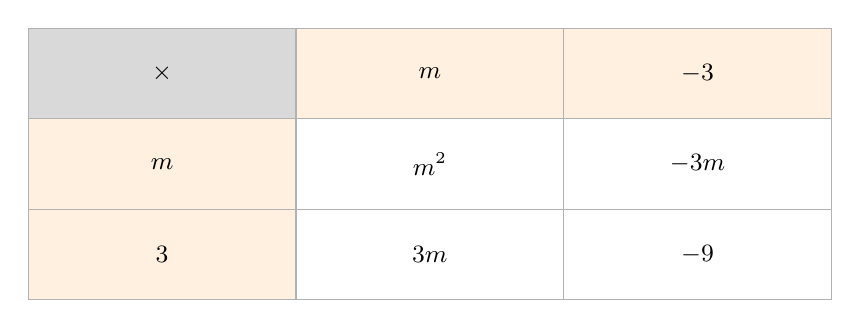
\begin{tikzpicture}[x=1cm,y=1cm,every node/.style={font=\small}]
\fill[gray!30] (0,0) rectangle (3.4,-1.15);
\draw[gray!60] (0,0) rectangle (3.4,-1.15);
\node at (1.7,-0.575) {$\displaystyle \times$};
\fill[orange!12] (3.4,0) rectangle (6.8,-1.15);
\draw[gray!60] (3.4,0) rectangle (6.8,-1.15);
\node at (5.1,-0.575) {$\displaystyle m$};
\fill[orange!12] (6.8,0) rectangle (10.2,-1.15);
\draw[gray!60] (6.8,0) rectangle (10.2,-1.15);
\node at (8.5,-0.575) {$\displaystyle -3$};
\fill[orange!12] (0,-1.15) rectangle (3.4,-2.3);
\draw[gray!60] (0,-1.15) rectangle (3.4,-2.3);
\node at (1.7,-1.725) {$\displaystyle m$};
\fill[white] (3.4,-1.15) rectangle (6.8,-2.3);
\draw[gray!60] (3.4,-1.15) rectangle (6.8,-2.3);
\node at (5.1,-1.725) {$\displaystyle m^2$};
\fill[white] (6.8,-1.15) rectangle (10.2,-2.3);
\draw[gray!60] (6.8,-1.15) rectangle (10.2,-2.3);
\node at (8.5,-1.725) {$\displaystyle -3m$};
\fill[orange!12] (0,-2.3) rectangle (3.4,-3.45);
\draw[gray!60] (0,-2.3) rectangle (3.4,-3.45);
\node at (1.7,-2.875) {$\displaystyle 3$};
\fill[white] (3.4,-2.3) rectangle (6.8,-3.45);
\draw[gray!60] (3.4,-2.3) rectangle (6.8,-3.45);
\node at (5.1,-2.875) {$\displaystyle 3m$};
\fill[white] (6.8,-2.3) rectangle (10.2,-3.45);
\draw[gray!60] (6.8,-2.3) rectangle (10.2,-3.45);
\node at (8.5,-2.875) {$\displaystyle -9$};
\end{tikzpicture}
\end{center}
\small Take out $5m$ first: $5m(m^2-9)$, then DOTS.\normalsize

\medskip\hrule

\section*{Factorising 43\quad\small\texttt{(a2-043)}}
\addcontentsline{toc}{section}{Factorising 43 (a2-043)}
\textit{Difficulty: Foundation \quad\textbar\quad Marks: 2}

\question{Factorise by grouping: \( cx + dx - cy - dy \)}

\textbf{Worked solution.}

\textit{Step 1: Group the first two terms and the last two terms, then factorise each pair. Be careful with the negative signs in the second pair.}
\[\begin{gathered}
x(c + d) - y(c + d)
\end{gathered}\]
Extract \( x \) from the first pair and \( -y \) from the second pair to ensure the inner brackets match.

\textit{Step 2: Factor out the newly formed common binomial bracket \( (c + d) \).}
\[\begin{gathered}
(c + d)(x - y)
\end{gathered}\]
Combine the factored groups together.

\begin{answerbox}
\textbf{Final answer:}\quad \(\displaystyle (c + d)(x - y)\)
\end{answerbox}
\textbf{Area-model diagram.}

\begin{center}
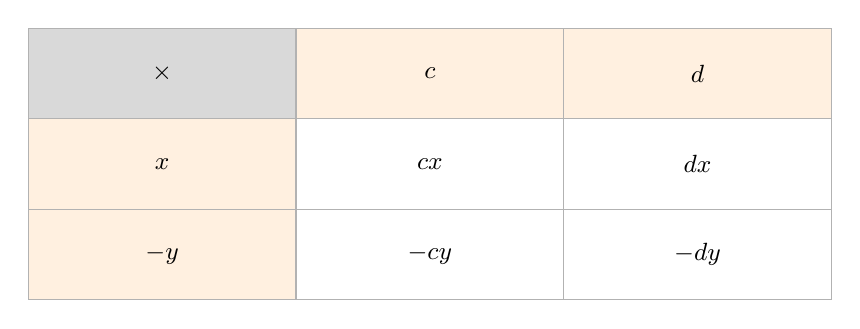
\begin{tikzpicture}[x=1cm,y=1cm,every node/.style={font=\small}]
\fill[gray!30] (0,0) rectangle (3.4,-1.15);
\draw[gray!60] (0,0) rectangle (3.4,-1.15);
\node at (1.7,-0.575) {$\displaystyle \times$};
\fill[orange!12] (3.4,0) rectangle (6.8,-1.15);
\draw[gray!60] (3.4,0) rectangle (6.8,-1.15);
\node at (5.1,-0.575) {$\displaystyle c$};
\fill[orange!12] (6.8,0) rectangle (10.2,-1.15);
\draw[gray!60] (6.8,0) rectangle (10.2,-1.15);
\node at (8.5,-0.575) {$\displaystyle d$};
\fill[orange!12] (0,-1.15) rectangle (3.4,-2.3);
\draw[gray!60] (0,-1.15) rectangle (3.4,-2.3);
\node at (1.7,-1.725) {$\displaystyle x$};
\fill[white] (3.4,-1.15) rectangle (6.8,-2.3);
\draw[gray!60] (3.4,-1.15) rectangle (6.8,-2.3);
\node at (5.1,-1.725) {$\displaystyle cx$};
\fill[white] (6.8,-1.15) rectangle (10.2,-2.3);
\draw[gray!60] (6.8,-1.15) rectangle (10.2,-2.3);
\node at (8.5,-1.725) {$\displaystyle dx$};
\fill[orange!12] (0,-2.3) rectangle (3.4,-3.45);
\draw[gray!60] (0,-2.3) rectangle (3.4,-3.45);
\node at (1.7,-2.875) {$\displaystyle -y$};
\fill[white] (3.4,-2.3) rectangle (6.8,-3.45);
\draw[gray!60] (3.4,-2.3) rectangle (6.8,-3.45);
\node at (5.1,-2.875) {$\displaystyle -cy$};
\fill[white] (6.8,-2.3) rectangle (10.2,-3.45);
\draw[gray!60] (6.8,-2.3) rectangle (10.2,-3.45);
\node at (8.5,-2.875) {$\displaystyle -dy$};
\end{tikzpicture}
\end{center}
\small Grouping: $x(c+d)-y(c+d)=(x-y)(c+d)$.\normalsize

\medskip\hrule

\section*{Factorising 44\quad\small\texttt{(a2-044)}}
\addcontentsline{toc}{section}{Factorising 44 (a2-044)}
\textit{Difficulty: Foundation \quad\textbar\quad Marks: 3}

\question{Simplify the expression, leaving your answer in factorised form: \( (2x+3)^2 - (2x+3)(x-1) \)}

\textbf{Worked solution.}

\textit{Step 1: Identify that \( (2x+3) \) is a common factor in both terms and extract it.}
\[\begin{gathered}
(2x+3)[(2x+3) - (x-1)]
\end{gathered}\]
Pull the shared binomial bracket out to the front.

\textit{Step 2: Carefully expand the inner expression, paying attention to the negative sign in front of the \( (x-1) \) bracket.}
\[\begin{gathered}
(2x+3)(2x + 3 - x + 1)
\end{gathered}\]
Distribute the negative sign to the terms inside the second bracket.

\textit{Step 3: Simplify the expression inside the second bracket by collecting like terms.}
\[\begin{gathered}
(2x+3)(x + 4)
\end{gathered}\]
Combine the \( x \) terms and the number terms.

\begin{answerbox}
\textbf{Final answer:}\quad \(\displaystyle (2x+3)(x+4)\)
\end{answerbox}
\textbf{Area-model diagram.}

\begin{center}
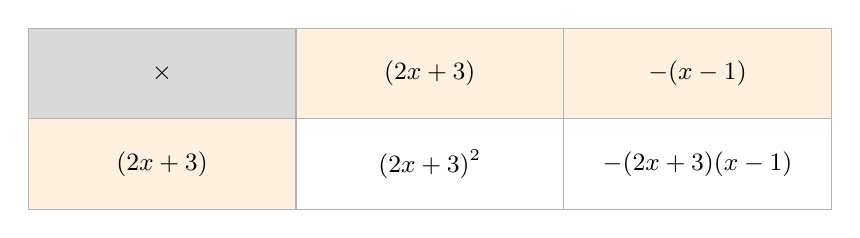
\begin{tikzpicture}[x=1cm,y=1cm,every node/.style={font=\small}]
\fill[gray!30] (0,0) rectangle (3.4,-1.15);
\draw[gray!60] (0,0) rectangle (3.4,-1.15);
\node at (1.7,-0.575) {$\displaystyle \times$};
\fill[orange!12] (3.4,0) rectangle (6.8,-1.15);
\draw[gray!60] (3.4,0) rectangle (6.8,-1.15);
\node at (5.1,-0.575) {$\displaystyle (2x+3)$};
\fill[orange!12] (6.8,0) rectangle (10.2,-1.15);
\draw[gray!60] (6.8,0) rectangle (10.2,-1.15);
\node at (8.5,-0.575) {$\displaystyle -(x-1)$};
\fill[orange!12] (0,-1.15) rectangle (3.4,-2.3);
\draw[gray!60] (0,-1.15) rectangle (3.4,-2.3);
\node at (1.7,-1.725) {$\displaystyle (2x+3)$};
\fill[white] (3.4,-1.15) rectangle (6.8,-2.3);
\draw[gray!60] (3.4,-1.15) rectangle (6.8,-2.3);
\node at (5.1,-1.725) {$\displaystyle (2x+3)^2$};
\fill[white] (6.8,-1.15) rectangle (10.2,-2.3);
\draw[gray!60] (6.8,-1.15) rectangle (10.2,-2.3);
\node at (8.5,-1.725) {$\displaystyle -(2x+3)(x-1)$};
\end{tikzpicture}
\end{center}
\small Common bracket $(2x+3)$; then $(2x+3)-(x-1)=(x+4)$.\normalsize

\medskip\hrule

\section*{Factorising 45\quad\small\texttt{(a2-045)}}
\addcontentsline{toc}{section}{Factorising 45 (a2-045)}
\textit{Difficulty: Foundation \quad\textbar\quad Marks: 1}

\question{Factorise: \( 12x - 18 \)}

\textbf{Worked solution.}

\textit{Find the highest common factor (HCF) of 12 and 18, which is 6.}
\[\begin{gathered}
6(2x - 3)
\end{gathered}\]
Divide both terms by 6 to find the expression inside the bracket.

\begin{answerbox}
\textbf{Final answer:}\quad \(\displaystyle 6(2x - 3)\)
\end{answerbox}
\textbf{Area-model diagram.}

\begin{center}
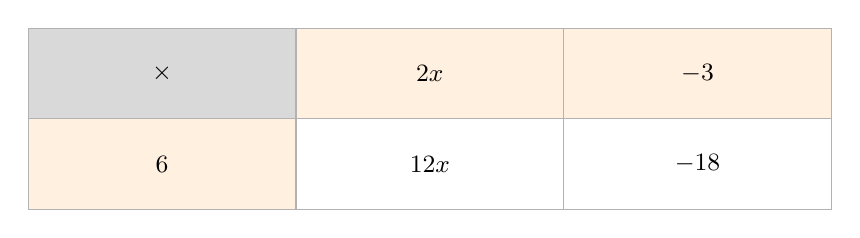
\begin{tikzpicture}[x=1cm,y=1cm,every node/.style={font=\small}]
\fill[gray!30] (0,0) rectangle (3.4,-1.15);
\draw[gray!60] (0,0) rectangle (3.4,-1.15);
\node at (1.7,-0.575) {$\displaystyle \times$};
\fill[orange!12] (3.4,0) rectangle (6.8,-1.15);
\draw[gray!60] (3.4,0) rectangle (6.8,-1.15);
\node at (5.1,-0.575) {$\displaystyle 2x$};
\fill[orange!12] (6.8,0) rectangle (10.2,-1.15);
\draw[gray!60] (6.8,0) rectangle (10.2,-1.15);
\node at (8.5,-0.575) {$\displaystyle -3$};
\fill[orange!12] (0,-1.15) rectangle (3.4,-2.3);
\draw[gray!60] (0,-1.15) rectangle (3.4,-2.3);
\node at (1.7,-1.725) {$\displaystyle 6$};
\fill[white] (3.4,-1.15) rectangle (6.8,-2.3);
\draw[gray!60] (3.4,-1.15) rectangle (6.8,-2.3);
\node at (5.1,-1.725) {$\displaystyle 12x$};
\fill[white] (6.8,-1.15) rectangle (10.2,-2.3);
\draw[gray!60] (6.8,-1.15) rectangle (10.2,-2.3);
\node at (8.5,-1.725) {$\displaystyle -18$};
\end{tikzpicture}
\end{center}
\small HCF $6$.\normalsize

\medskip\hrule

\section*{Factorising 46\quad\small\texttt{(a2-046)}}
\addcontentsline{toc}{section}{Factorising 46 (a2-046)}
\textit{Difficulty: Foundation \quad\textbar\quad Marks: 2}

\question{Factorise fully: \( 5a^2b + 10ab^2 \)}

\textbf{Worked solution.}

\textit{Step 1: Identify the highest common numerical factor (which is 5) and the shared variables (which are \( a \) and \( b \)).}
\[\begin{gathered}
5ab
\end{gathered}\]
Find the greatest term that divides exactly into both parts of the expression.

\textit{Step 2: Factor out \( 5ab \) from the original expression.}
\[\begin{gathered}
5ab(a + 2b)
\end{gathered}\]
Divide each original term by the common factor to populate the bracket.

\begin{answerbox}
\textbf{Final answer:}\quad \(\displaystyle 5ab(a + 2b)\)
\end{answerbox}
\textbf{Area-model diagram.}

\begin{center}
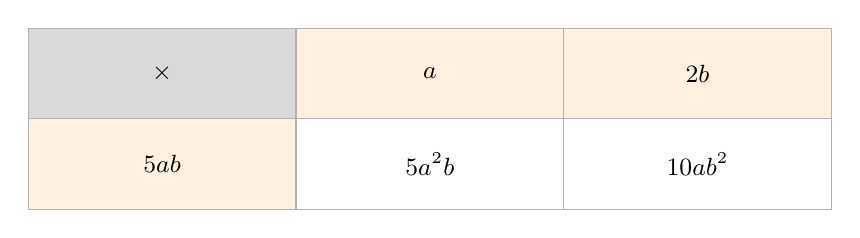
\begin{tikzpicture}[x=1cm,y=1cm,every node/.style={font=\small}]
\fill[gray!30] (0,0) rectangle (3.4,-1.15);
\draw[gray!60] (0,0) rectangle (3.4,-1.15);
\node at (1.7,-0.575) {$\displaystyle \times$};
\fill[orange!12] (3.4,0) rectangle (6.8,-1.15);
\draw[gray!60] (3.4,0) rectangle (6.8,-1.15);
\node at (5.1,-0.575) {$\displaystyle a$};
\fill[orange!12] (6.8,0) rectangle (10.2,-1.15);
\draw[gray!60] (6.8,0) rectangle (10.2,-1.15);
\node at (8.5,-0.575) {$\displaystyle 2b$};
\fill[orange!12] (0,-1.15) rectangle (3.4,-2.3);
\draw[gray!60] (0,-1.15) rectangle (3.4,-2.3);
\node at (1.7,-1.725) {$\displaystyle 5ab$};
\fill[white] (3.4,-1.15) rectangle (6.8,-2.3);
\draw[gray!60] (3.4,-1.15) rectangle (6.8,-2.3);
\node at (5.1,-1.725) {$\displaystyle 5a^2b$};
\fill[white] (6.8,-1.15) rectangle (10.2,-2.3);
\draw[gray!60] (6.8,-1.15) rectangle (10.2,-2.3);
\node at (8.5,-1.725) {$\displaystyle 10ab^2$};
\end{tikzpicture}
\end{center}
\small HCF $5ab$.\normalsize

\medskip\hrule

\section*{Factorising 47\quad\small\texttt{(a2-047)}}
\addcontentsline{toc}{section}{Factorising 47 (a2-047)}
\textit{Difficulty: Foundation \quad\textbar\quad Marks: 2}

\question{Write the expression as a product of factors: \( 81p^2 - 16q^2 \)}

\textbf{Worked solution.}

\textit{Recognise this as a difference of two squares, rewriting the terms as \( (9p)^2 \) and \( (4q)^2 \).}
\[\begin{gathered}
(9p)^2 - (4q)^2
\end{gathered}\]
Identify the squared components to apply the rule \( A^2 - B^2 = (A-B)(A+B) \).

\begin{answerbox}
\textbf{Final answer:}\quad \(\displaystyle (9p - 4q)(9p + 4q)\)
\end{answerbox}
\textbf{Area-model diagram.}

\begin{center}
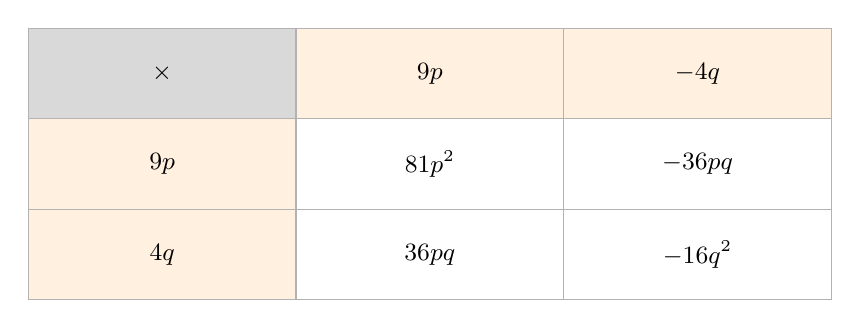
\begin{tikzpicture}[x=1cm,y=1cm,every node/.style={font=\small}]
\fill[gray!30] (0,0) rectangle (3.4,-1.15);
\draw[gray!60] (0,0) rectangle (3.4,-1.15);
\node at (1.7,-0.575) {$\displaystyle \times$};
\fill[orange!12] (3.4,0) rectangle (6.8,-1.15);
\draw[gray!60] (3.4,0) rectangle (6.8,-1.15);
\node at (5.1,-0.575) {$\displaystyle 9p$};
\fill[orange!12] (6.8,0) rectangle (10.2,-1.15);
\draw[gray!60] (6.8,0) rectangle (10.2,-1.15);
\node at (8.5,-0.575) {$\displaystyle -4q$};
\fill[orange!12] (0,-1.15) rectangle (3.4,-2.3);
\draw[gray!60] (0,-1.15) rectangle (3.4,-2.3);
\node at (1.7,-1.725) {$\displaystyle 9p$};
\fill[white] (3.4,-1.15) rectangle (6.8,-2.3);
\draw[gray!60] (3.4,-1.15) rectangle (6.8,-2.3);
\node at (5.1,-1.725) {$\displaystyle 81p^2$};
\fill[white] (6.8,-1.15) rectangle (10.2,-2.3);
\draw[gray!60] (6.8,-1.15) rectangle (10.2,-2.3);
\node at (8.5,-1.725) {$\displaystyle -36pq$};
\fill[orange!12] (0,-2.3) rectangle (3.4,-3.45);
\draw[gray!60] (0,-2.3) rectangle (3.4,-3.45);
\node at (1.7,-2.875) {$\displaystyle 4q$};
\fill[white] (3.4,-2.3) rectangle (6.8,-3.45);
\draw[gray!60] (3.4,-2.3) rectangle (6.8,-3.45);
\node at (5.1,-2.875) {$\displaystyle 36pq$};
\fill[white] (6.8,-2.3) rectangle (10.2,-3.45);
\draw[gray!60] (6.8,-2.3) rectangle (10.2,-3.45);
\node at (8.5,-2.875) {$\displaystyle -16q^2$};
\end{tikzpicture}
\end{center}
\small DOTS: $81p^2=(9p)^2,\ 16q^2=(4q)^2$.\normalsize

\medskip\hrule

\section*{Factorising 48\quad\small\texttt{(a2-048)}}
\addcontentsline{toc}{section}{Factorising 48 (a2-048)}
\textit{Difficulty: Foundation \quad\textbar\quad Marks: 2}

\question{Express as the product of factors: \( 2x(y-1) + 3(y-1) \)}

\textbf{Worked solution.}

\textit{Identify that the binomial \( (y-1) \) is a common factor in both terms.}
\[\begin{gathered}
(y-1)(2x + 3)
\end{gathered}\]
Extract the shared bracket to the front and group the remaining outer terms into a second bracket.

\begin{answerbox}
\textbf{Final answer:}\quad \(\displaystyle (y-1)(2x + 3)\)
\end{answerbox}
\textbf{Area-model diagram.}

\begin{center}
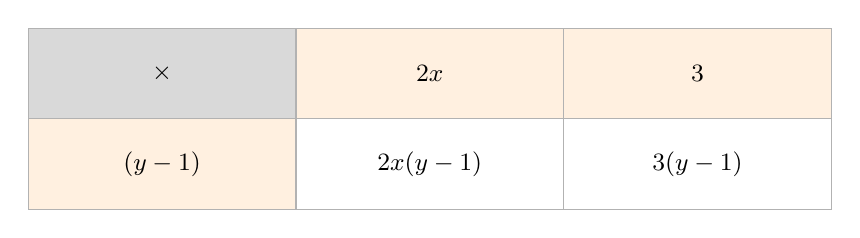
\begin{tikzpicture}[x=1cm,y=1cm,every node/.style={font=\small}]
\fill[gray!30] (0,0) rectangle (3.4,-1.15);
\draw[gray!60] (0,0) rectangle (3.4,-1.15);
\node at (1.7,-0.575) {$\displaystyle \times$};
\fill[orange!12] (3.4,0) rectangle (6.8,-1.15);
\draw[gray!60] (3.4,0) rectangle (6.8,-1.15);
\node at (5.1,-0.575) {$\displaystyle 2x$};
\fill[orange!12] (6.8,0) rectangle (10.2,-1.15);
\draw[gray!60] (6.8,0) rectangle (10.2,-1.15);
\node at (8.5,-0.575) {$\displaystyle 3$};
\fill[orange!12] (0,-1.15) rectangle (3.4,-2.3);
\draw[gray!60] (0,-1.15) rectangle (3.4,-2.3);
\node at (1.7,-1.725) {$\displaystyle (y-1)$};
\fill[white] (3.4,-1.15) rectangle (6.8,-2.3);
\draw[gray!60] (3.4,-1.15) rectangle (6.8,-2.3);
\node at (5.1,-1.725) {$\displaystyle 2x(y-1)$};
\fill[white] (6.8,-1.15) rectangle (10.2,-2.3);
\draw[gray!60] (6.8,-1.15) rectangle (10.2,-2.3);
\node at (8.5,-1.725) {$\displaystyle 3(y-1)$};
\end{tikzpicture}
\end{center}
\small Common bracket $(y-1)$.\normalsize

\medskip\hrule

\section*{Factorising 49\quad\small\texttt{(a2-049)}}
\addcontentsline{toc}{section}{Factorising 49 (a2-049)}
\textit{Difficulty: Foundation \quad\textbar\quad Marks: 3}

\question{Express as the product of factors: \( m(n-3) - 2(3-n) \)}

\textbf{Worked solution.}

\textit{Step 1: Notice the brackets \( (n-3) \) and \( (3-n) \) are opposites. Factor out -1 from the second term to make them identical.}
\[\begin{gathered}
m(n-3) + 2(n-3)
\end{gathered}\]
Reverse the sign of the second term to reveal a common bracket.

\textit{Step 2: Factor out the common bracket \( (n-3) \).}
\[\begin{gathered}
(n-3)(m + 2)
\end{gathered}\]
Extract the shared binomial factor.

\begin{answerbox}
\textbf{Final answer:}\quad \(\displaystyle (n-3)(m + 2)\)
\end{answerbox}
\textbf{Area-model diagram.}

\begin{center}
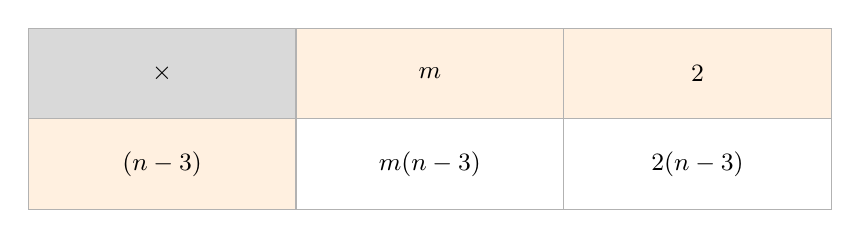
\begin{tikzpicture}[x=1cm,y=1cm,every node/.style={font=\small}]
\fill[gray!30] (0,0) rectangle (3.4,-1.15);
\draw[gray!60] (0,0) rectangle (3.4,-1.15);
\node at (1.7,-0.575) {$\displaystyle \times$};
\fill[orange!12] (3.4,0) rectangle (6.8,-1.15);
\draw[gray!60] (3.4,0) rectangle (6.8,-1.15);
\node at (5.1,-0.575) {$\displaystyle m$};
\fill[orange!12] (6.8,0) rectangle (10.2,-1.15);
\draw[gray!60] (6.8,0) rectangle (10.2,-1.15);
\node at (8.5,-0.575) {$\displaystyle 2$};
\fill[orange!12] (0,-1.15) rectangle (3.4,-2.3);
\draw[gray!60] (0,-1.15) rectangle (3.4,-2.3);
\node at (1.7,-1.725) {$\displaystyle (n-3)$};
\fill[white] (3.4,-1.15) rectangle (6.8,-2.3);
\draw[gray!60] (3.4,-1.15) rectangle (6.8,-2.3);
\node at (5.1,-1.725) {$\displaystyle m(n-3)$};
\fill[white] (6.8,-1.15) rectangle (10.2,-2.3);
\draw[gray!60] (6.8,-1.15) rectangle (10.2,-2.3);
\node at (8.5,-1.725) {$\displaystyle 2(n-3)$};
\end{tikzpicture}
\end{center}
\small Rewrite $-2(3-n)=+2(n-3)$ to expose the common bracket $(n-3)$.\normalsize

\medskip\hrule

\section*{Factorising 50\quad\small\texttt{(a2-050)}}
\addcontentsline{toc}{section}{Factorising 50 (a2-050)}
\textit{Difficulty: Foundation \quad\textbar\quad Marks: 3}

\question{Factorise completely: \( 18x^2 - 50 \)}

\textbf{Worked solution.}

\textit{Step 1: Extract the highest common numerical factor of 2 from both terms first.}
\[\begin{gathered}
2(9x^2 - 25)
\end{gathered}\]
Always check for a common factor before applying difference of two squares.

\textit{Step 2: Recognise that the expression inside the bracket is a difference of two squares and factorise it.}
\[\begin{gathered}
2(3x - 5)(3x + 5)
\end{gathered}\]
Apply the pattern \( A^2 - B^2 = (A-B)(A+B) \) to the inner quadratic.

\begin{answerbox}
\textbf{Final answer:}\quad \(\displaystyle 2(3x - 5)(3x + 5)\)
\end{answerbox}
\textbf{Area-model diagram.}

\begin{center}
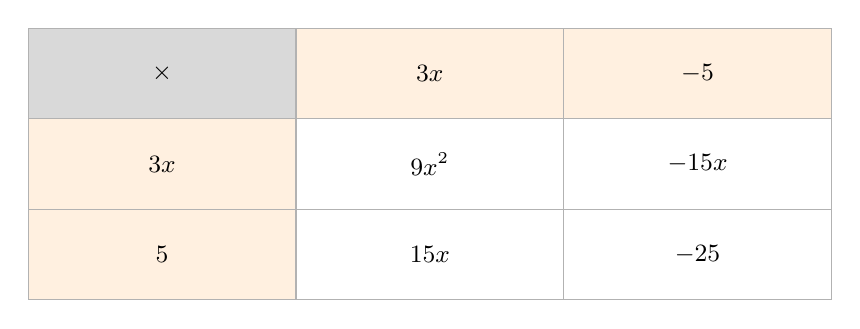
\begin{tikzpicture}[x=1cm,y=1cm,every node/.style={font=\small}]
\fill[gray!30] (0,0) rectangle (3.4,-1.15);
\draw[gray!60] (0,0) rectangle (3.4,-1.15);
\node at (1.7,-0.575) {$\displaystyle \times$};
\fill[orange!12] (3.4,0) rectangle (6.8,-1.15);
\draw[gray!60] (3.4,0) rectangle (6.8,-1.15);
\node at (5.1,-0.575) {$\displaystyle 3x$};
\fill[orange!12] (6.8,0) rectangle (10.2,-1.15);
\draw[gray!60] (6.8,0) rectangle (10.2,-1.15);
\node at (8.5,-0.575) {$\displaystyle -5$};
\fill[orange!12] (0,-1.15) rectangle (3.4,-2.3);
\draw[gray!60] (0,-1.15) rectangle (3.4,-2.3);
\node at (1.7,-1.725) {$\displaystyle 3x$};
\fill[white] (3.4,-1.15) rectangle (6.8,-2.3);
\draw[gray!60] (3.4,-1.15) rectangle (6.8,-2.3);
\node at (5.1,-1.725) {$\displaystyle 9x^2$};
\fill[white] (6.8,-1.15) rectangle (10.2,-2.3);
\draw[gray!60] (6.8,-1.15) rectangle (10.2,-2.3);
\node at (8.5,-1.725) {$\displaystyle -15x$};
\fill[orange!12] (0,-2.3) rectangle (3.4,-3.45);
\draw[gray!60] (0,-2.3) rectangle (3.4,-3.45);
\node at (1.7,-2.875) {$\displaystyle 5$};
\fill[white] (3.4,-2.3) rectangle (6.8,-3.45);
\draw[gray!60] (3.4,-2.3) rectangle (6.8,-3.45);
\node at (5.1,-2.875) {$\displaystyle 15x$};
\fill[white] (6.8,-2.3) rectangle (10.2,-3.45);
\draw[gray!60] (6.8,-2.3) rectangle (10.2,-3.45);
\node at (8.5,-2.875) {$\displaystyle -25$};
\end{tikzpicture}
\end{center}
\small Take out $2$ first: $2(9x^2-25)$, then DOTS.\normalsize

\medskip\hrule

\end{document}
